\documentclass[titlepage,a4paper]{article}

\usepackage{a4wide}
\usepackage[colorlinks=true,linkcolor=black,urlcolor=blue,bookmarksopen=true]{hyperref}
\usepackage{bookmark}
\usepackage{fancyhdr}
\usepackage[spanish]{babel}
\usepackage[utf8]{inputenc}
\usepackage[T1]{fontenc}
\usepackage{graphicx}
\usepackage{float}
\usepackage[table,xcdraw]{xcolor}
\pagestyle{fancy} % Encabezado y pie de página
\fancyhf{}
\fancyhead[L]{Apuntes Análisis de la información}
\fancyhead[R]{1C2021}
\renewcommand{\headrulewidth}{0.4pt}
\fancyfoot[C]{\thepage}
\renewcommand{\footrulewidth}{0.4pt}

\begin{document}
\begin{titlepage} % Carátula
	\hfill
\includegraphics[width=6cm]{logofiuba.jpg}
    \centering
    \vfill
    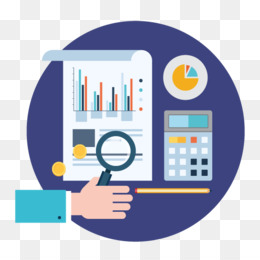
\includegraphics[width=6cm]{Imagenes/logo.jpg}
    
    \Huge \textbf{Apuntes de}
    
    \Huge \textbf{Análisis de la Información}
    \vskip2cm
    \Large [7509]\\
    Curso González \\
    1C 2021 
    \vfill
    \begin{tabular}{ | l | }
      \hline
      Grassano, Bruno \\ \hline
      bgrassano@fi.uba.ar \\ \hline
  	\end{tabular}
    \vfill
    \vfill
\end{titlepage}

\tableofcontents % Índice general

\newpage

\section{Introducción}\label{sec:intro}
El presente archivo contiene los apuntes que fueron tomados a lo largo de la cursada de la materia análisis de la información (7509) en el curso del profesor González - Turri.

\subsection*{Recomendaciones}
La materia es muy tranquila y buena parte de los contenidos ya se tiene una idea de antes, sobretodo si se esta trabajando. (En mi opinión esta materia quedaría mejor al comienzo de la carrera)

Respecto a los trabajos prácticos, son 3 (este cuatrimestre en virtualidad) y se realizan en grupos de 5/6. En los tres se realiza el mismo proceso de análisis de requisitos y una propuesta de mejora con Lean UX, no se programan los sistemas. En los dos primeros se entrega el documento con todo lo realizado, y en el tercero se realiza una presentación como preparación para el final. No requieren mucho tiempo cada uno. 

El final consiste en realizar otro análisis de requisitos y mejora pero sin el acompañamiento del profesor de la practica, este trabajo se expone en una presentación, y luego se realizan preguntas teóricas de forma individual.

% Grupos 5/6
% Final exposición de TP para coloquio. Evaluación de la exposición, calidad del trabajo, presentación, algunas preguntas teóricas individuales (solo sobre lo de los lunes)
% Nota final: Conceptual (Alejandro sobre el trabajo) + Exposición + Respuestas a preguntas teóricas

\newpage

\section*{Primera clase}
\section{Introducción a la Ing. Software}
Definición: \textit{'Es la aplicación de un enfoque sistemático disciplinado y cuantificable al desarrollo, operación y mantenimiento de productos de software.'} (IEEE 1993) (Enfoque ingenieril)

\medskip

Otra definición: \textit{'Comprende principios y \textbf{metodologías} para desarrollar, operar y mantener software de calidad.'}


\subsection{Metodologías}
Contiene 3 partes. Los modelos, procesos, y las herramientas de un desarrollo de software. Estos son específicos a una metodología.

    \begin{itemize}
        \item Los modelos necesitan de un lenguaje de modelado $\rightarrow$ UML.
        \item Los procesos son \textit{XP, SCRUM, RUP, etc}
        \item Herramientas \textit{Suite Rational}
    \end{itemize}
    
    \begin{figure}[!htb]
        \centering
        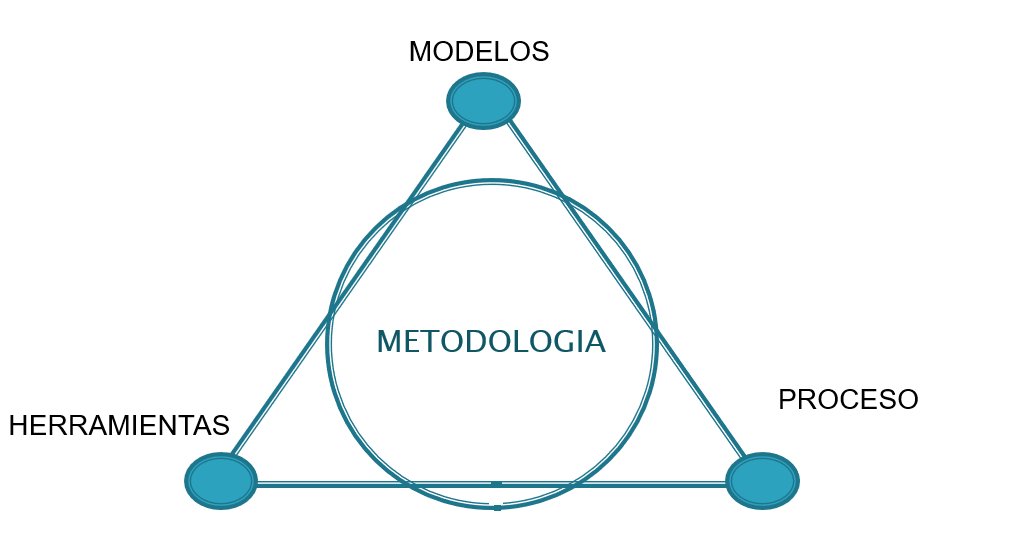
\includegraphics[width=0.8\textwidth]{Imagenes/Metodologias.png}
        \caption{Composición de una metodología}
    \end{figure}

\subsection{Modelos}


\begin{figure}[!htb]
    \centering
    \hspace*{-2.8cm}
    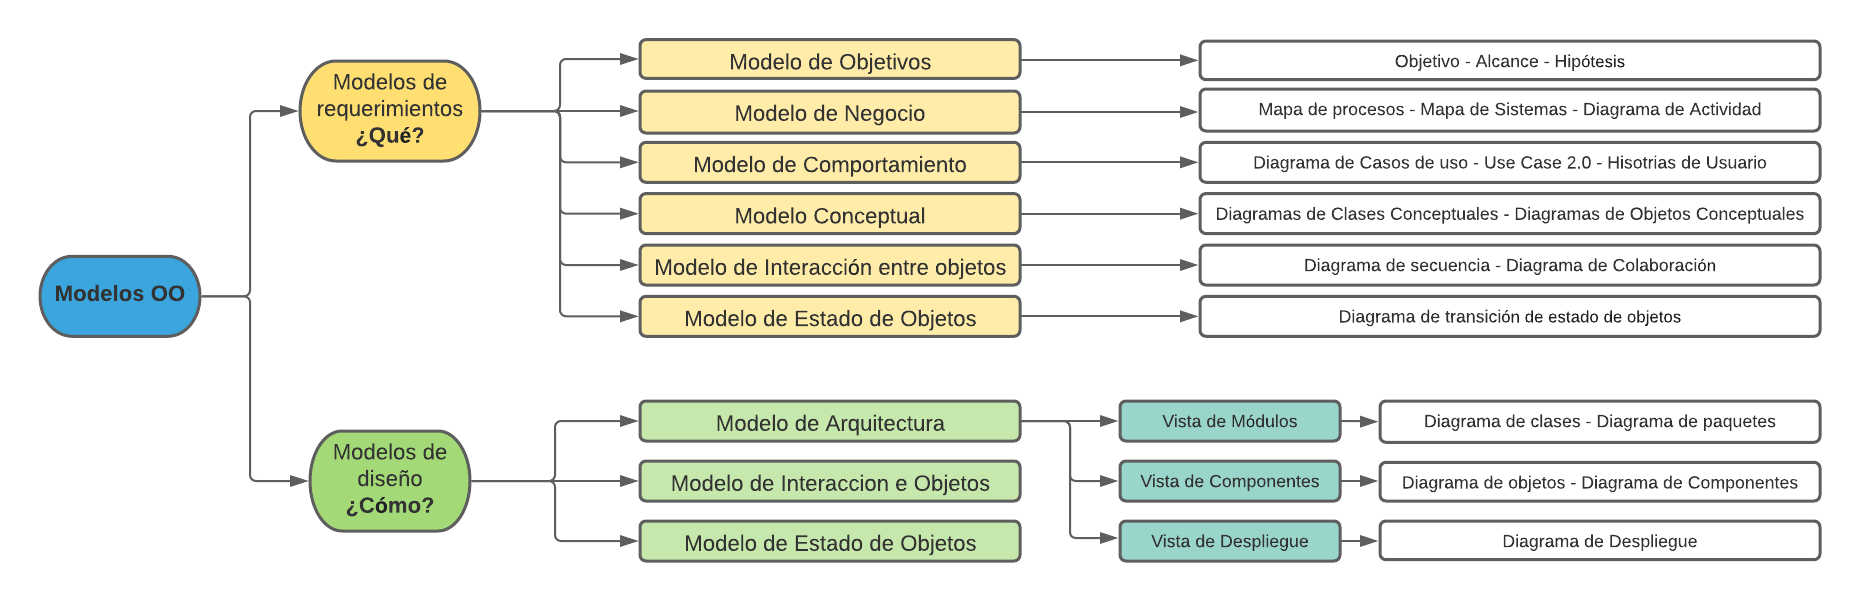
\includegraphics[width=1.3\textwidth]{Imagenes/ModelosOO.png}
    \caption{Modelos OO diferenciados en los tipos del QUE y del COMO}
\end{figure}

\subsubsection*{¿Que es un modelo?}
Es una simplificación de la realidad. Como la realidad es compleja le aplicamos abstracción, para incluir elementos que tienen mucha influencia y omitir los relevantes.

\subsubsection*{¿Para que sirve un modelo?}
    \begin{itemize}
        \item Para comprender mejor el sistema que estamos desarrollando.
        \item Para poder comunicarnos, con el cliente y el equipo de diseño.
        \item Visualizar y controlar rápidamente la arquitectura del sistema.
        \item Gestionar el riesgo de un proyecto. \textit{Calidad, plazos, y presupuesto}
    \end{itemize}

\subsubsection*{Etapas}
    \begin{itemize}
        \item Captura de requerimientos. \textit{Reuniones con cliente, cuestionarios, focus groups,...}
        \item Análisis de requerimientos: Es el ¿Que se necesita? \textit{Modelos de casos de uso, historias de usuario,...}
        \item Diseño: Es el ¿Como voy a hacer? \textit{Modelos de clases, de objetos, de despliegue,...}
        \item Construcción. \textit{Programación, integración de componentes...}
        \item Pruebas. \textit{Pruebas de sistema, unitarias, de usuario, de integración}
        \item Entrega. \textit{Despliegue del producto a los usuarios}
        \item Mantenimiento. \textit{Correctivo (Corregir defectos de diseño) y evolutivo (Adaptar a los nuevos procesos)}
    \end{itemize}

\subsubsection*{Principios de la modelización}
    \begin{itemize}
        \item La elección de que modelos crear tiene una gran influencia sobre como se aborda un problema y como se da la solución.
        \item Tienen distintos niveles de precisión.
        \item Los mejores modelos tienen que estar ligados a la realidad.
        \item Un único modelo no es suficiente.
        \item Tener un Objetivo y alcance claro.
    \end{itemize}

\subsubsection*{Beneficios de la modelización}
    \begin{itemize}
        \item Forma de visualizar necesidades y requerimientos contra costos reales antes de comenzar el desarrollo.
        \item Se trabaja en un alto nivel de abstracción
    \end{itemize}


\subsubsection*{Enfoques}
    \begin{itemize}
        \item Algorítmico
        \item Orientado a objetos
    \end{itemize}

\subsection{Paradigma orientado a objetos}
    \begin{itemize}
        \item Esta basado en la creación de componentes reutilizables.
        \item Construcción de software mas rápida y dinámica.
        \item Facilita la creación de prototipos.
    \end{itemize}

\subsection{UML}
Es un \textbf{lenguaje} estándar para escribir 'planos' de software. Lenguaje para visualizar, especificar, construir y documentar sistemas bajo el paradigma de orientación a objetos. Se utiliza desde el inicio hasta el fin del proyecto.
\textbf{No} es una \textbf{metodología}.

    \begin{figure}[!htb]
        \centering
        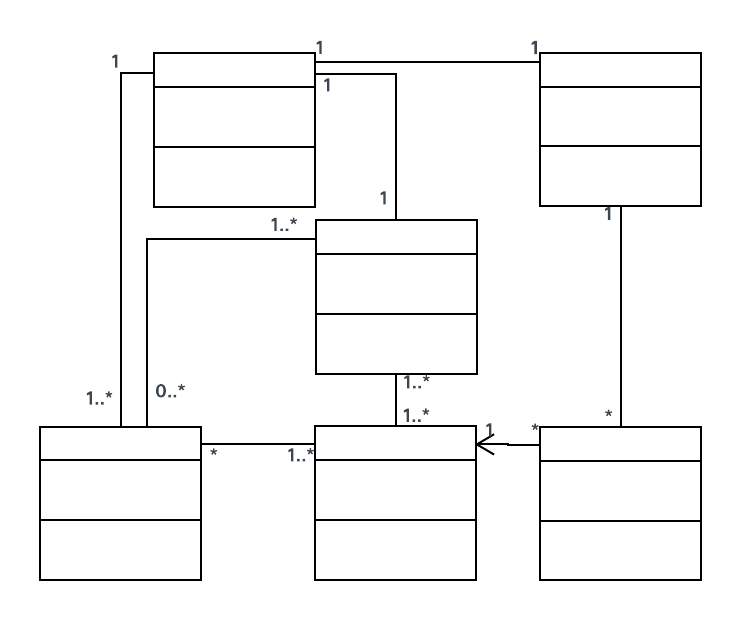
\includegraphics[width=0.5\textwidth]{Imagenes/UML.png}
    \end{figure}

\subsection*{Aspectos del modelado}
    \begin{itemize}
        \item Modelado funcional o de comportamiento. \textit{Historias de usuario}
        \item Modelado estático o estructural. \textit{Diagrama de clases}
        \item Modelado dinámico. \textit{Diagramas de interacción, secuencia}
    \end{itemize}

\subsection{Procesos de desarrollo de software}

Tiene que responder a 4 preguntas: ¿Quien lo hace?, ¿Que lo hace?, ¿Como lo hace?, ¿Cuando lo hace?
De forma tal de obtener un producto de calidad, dentro de plazos y presupuestos predecibles.

\section{Modelo de Objetivos}
Dentro de los modelos de requerimientos.
\subsection{Objetivo del sistema}
Define lo que el sistema va a hacer (objetivo).
Es una descripción breve con alto nivel de abstracción, sobre \textbf{que} se requiere automatizar con el sistema, declarando los 'macroprocesos'.

\textit{Ej.
El sistema esta dirigido a administrar las ventas de la empresa, incluyendo la gestión de los pedidos del stock y la facturación de las mismas'.}

Macroprocesos involucrados: Gestión de pedidos, gestión de stock, gestión de facturación.

\subsection{Alcance del sistema}
Muestra los limites del objetivo(alcance). Para cada 'macroprocesos' hay que indicar las funcionalidades que el sistema va a contemplar,
dejando bien en claro que funcionalidades están \underline{dentro}/\underline{fuera} del alcance

Formato típico de un análisis del alcance.



\begin{table}[]
\begin{center}
\begin{tabular}{|l|l|c|}
\hline
\multicolumn{1}{|c|}{Macroproceso} & \multicolumn{1}{c|}{Funcionalidades} & Alcance \\ \hline
\textit{Nombre macroproceso}      & \textit{Nombre funcionalidad}       & \textit{Si/No} \\ \hline
 \multicolumn{1}{|c|}{...}          & \multicolumn{1}{c|}{...}            & ...            \\ \hline
\end{tabular}
\end{center}
\end{table}


\subsection{Hipótesis o supuestos funcionales}
Establece premisas o restricciones a tener en cuenta. (hipótesis)
Pueden ser establecidas por políticas de la empresa, normativas legales. Supuestos iniciales establecidos por el analista (deben ser verificados después por el cliente). No son requerimientos relevados, sino que complementan a los mismos.

Estos pueden darse por falta de relevamiento por determinadas circunstancias. \textit{Ej. El cliente se lo olvido, es trivial, no lo sabe, lo oculta}

\subsection{Caso de estudio: Airbus A320}

Habilitar la aceleración en reversa. El avión al momento de frenar activa este mecanismo, abriendo unos alerones en las turbinas.

El software: el piloto acciona el comando, ocurre un servo-mecanismo que abre los alerones. Caso de error a evitar, si el piloto lo acciona volando, tiene que haber algún mecanismo que detecte que el avión este en el piso. Se agrego un sensor de giro de ruedas, que detecta cuando giran en el piso y habilita la reversa del sistema que acciono el piloto.

El software salio de esta forma, pero tenia un problema, el avión estaba aterrizando, pero en caso de que la pista tenga hielo se producía un bloqueo y la rueda patinaba en vez de girar. Esto pasó debido a que no se contemplo en el universo en estudio.

Se debería de haber tenido en cuenta el sensor de giro, de peso, y de altura.

Sistema de estudio: software, los 3 sensores, el servo-mecanismo reversa.

\newpage
\section*{Segunda clase}
\section{Modelo de negocio}
Dentro de los modelos de requerimientos.
\subsection{Mapa de procesos}
    \begin{itemize}
        \item Modeliza los procesos que una organización tiene para llevar adelante sus funciones.
        \item Permite entender la organización/negocio.
        \item Es un modelo matricial, modela los principales macroprocesos necesarios para el funcionamiento del negocio/empresa.
        \item Columnas: áreas del negocio. \textit{Ej. Estrategia y planificación, operación, previsión, assurance, billing}
        \item Filas: visión por capas. \textit{Ej. cliente, servicio, recurso, enterprise}
    \end{itemize}
    
    
    Conocer aquellos que vamos a automatizar, mas aquellos que interaccionan con el mismo.
    
\subsection{Mapa de sistemas}
    \begin{itemize}
        \item Modelo matricial: incluye los sistemas que dan soporte a los procesos de negocio.
        \item Columnas: áreas del negocio
        \item Filas: visión por capas
    \end{itemize}

Mapea determinados macroprocesos, y va diciendo cuales son los sistemas que van a automatizar los macroprocesos (mapa de sistemas) Puede ser mapeo 1 a 1, 1 a N, N a 1.

\subsection{Diagrama de actividad}
    \begin{itemize}
        \item Modeliza una secuencia de actividades en un escenario determinado. Modelo gráfico.
        \item Esta compuesto por un grafo dirigido. Los nodos son actividades, y los arcos (dirigidos) representan la transición entre actividades.
        \item Actividad de inicio, es única (circulo relleno) 
        \item Actividades de fin, puede haber varias (circulo con borde)
        \item El rombo (bifurcación) es de decisión. Indica caminos alternativos, elegidos según el valor de alguna expresión, surgida de un análisis que se lleva a cabo en una actividad.
        \item Barra de sincronización, agregar la barra indica que para que inicie otra actividad, tienen que haber finalizado todas las actividades que vayan a la barra.
        \item Dividiendo como columnas, agregar los responsables de cada actividad, quien las ejecuta. (Las 'Swimming lines', carriles, dividen las actividades')
        \item Estos diagramas no muestran temporalidad, esto esta en diagramas de secuencia.
        \item No muestran requisitos NO funcionales.
        \item Muy claro para comunicarse con el cliente y asegurarse de que se entendieron los requerimientos.
        \item Buen punto de partida para generar el modelo de comportamiento.
        \item Tipos de escenarios
        \begin{itemize}
            \item Global, contiene todos los procesos de negocio del universo en estudio.
            \item Parte del negocio, contiene algunos procesos de negocio del universo en estudio
            \item Un solo proceso de negocio, tiene todas las actividades de ese proceso.
            \item Regla de negocio, son las actividades de una regla de negocio.
        \end{itemize}
    \end{itemize}

    \begin{figure}[!htb]
        \centering
        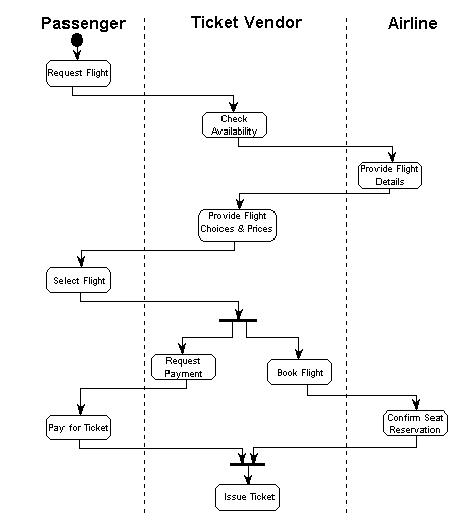
\includegraphics[width=0.7\textwidth]{Imagenes/DiagramaActividad.png}
        \caption{Diagrama de actividad. Notar las diferentes entidades: Actores, actividad de inicio (de fin falta), las secuencias, barras de sincronización.}
    \end{figure}

Una actividad esta compuesta por un conjunto de tareas a ser realizadas. Verbo $+$ objeto, \textit{ej. verificar pedido}. No hay que asociarlas con actividades físicas, si con procesos y/o reglas de negocio que luego podrán ser (o no) automatizadas.


\newpage
\section*{Tercera y cuarta clase}

\section{Modelo de comportamiento}
Dentro de los modelos de requerimientos.

\subsection{Casos de uso}
Hay tres componentes en el modelo de comportamiento.
\begin{itemize}
    \item Actores, representa algo o alguien (una persona, dispositivo, otro sistema) que interactúa con el sistema sin ser parte de el. Puede ingresar y/o recibir información del sistema. Se identifican fácilmente a partir de los roles representados por la swimline's. Se pueden identificar respondiendo a las siguientes preguntas: ¿Quien esta interesado en cierto requerimiento? ¿En que lugar de la organización se usa el sistema? ¿Quien se beneficiara con el uso del sistema? ¿Quien mantendrá el sistema? Etc.
    
    La clave para identificar buenos actores es pensar en el rol con el cual el actor interacciona con el sistema.

    \item Casos de uso, especifica el comportamiento de una parte del sistema. Representan un \textbf{requisito funcional} del sistema. Es un conjunto de acciones (variaciones incluidas) que ejecuta un sistema para producir un resultado para un actor. Gráficamente es una elipse con el nombre del caso de uso adentro.
    
    Son fácilmente identificables a partir del modelo de negocio (las actividades/tareas). Se pueden identificar con algunas preguntas también. ¿Cuales son las tareas de cada actor? ¿Que casos de uso crecerán, almacenaran, modificaran, consultaran, o eliminaran esta información? ¿Algún actor necesita informar al sistema sobre cambios externos? ¿Necesita algún actor ser informado de cambios en el sistema? Etc.
    
    Para identificar buenos y malos casos de uso, hay dos reglas.
    \begin{itemize}
        \item Completitud temporal, un caso de uso debe ser completo de principio a fin. \textit{Ej. Malos casos: seleccionar curso, registrar curso, informar registro (no son completos de principio a fin, cada uno esta en una parte, alumno, sistema)- Correcto: Registrar curso. (va del alumno al sistema)}
        \item completitud funcional, cuando varios casos de uso tratan con la misma entidad y son iniciados por el mismo actor podemos resumirlo en un solo caso de uso.\textit{Ej. Incorrecto: Departamento alumno: agregar curso, modificar curso, eliminar curso - Correcto: Mantener curso}
    \end{itemize}
    
    \item Diagramas de casos de uso, muestrea un conjunto de casos de uso, actores y sus relaciones. Permite tener una visualización del comportamiento de un sistema. En los diagramas de caso de uso general, se tiene una visión de alto nivel de todo el sistema, hay que tener 'todos' los actores y 'todos' los casos de uso del sistema. Hay actores primarios (izquierda diagrama)(disparan casos de uso) y actores secundarios (derecha diagrama)(no disparan casos de uso). Puede darse que un actor sea principal y secundario (esta en ambos lados).
\end{itemize}

\begin{figure}[!htb]
    \centering
    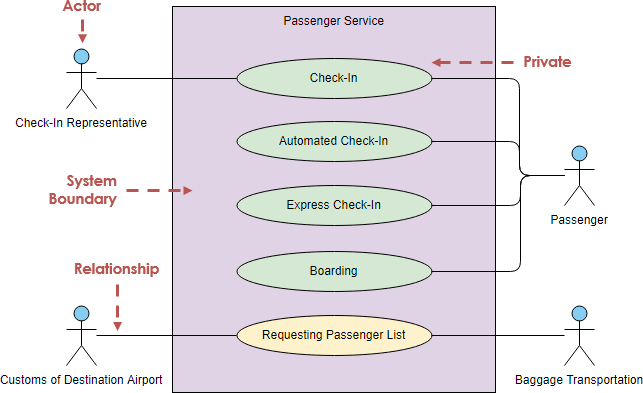
\includegraphics[width=0.9 \textwidth]{Imagenes/CasoDeUso.png}
    \caption{Ejemple de diagrama de casos de uso.}
\end{figure}


\subsection{Documentación de casos de uso}
Tienen una descripción del caso, y flujo de eventos. (pre-condiciones, flujo principal, subflujos, flujos de excepción, post-condiciones)

Las pre-condiciones son las acciones que deben haber sido ejecutadas previas a la ejecución del caso de uso. 

Flujo de eventos, es una descripción de una secuencia de acciones necesarias para proveer la funcionalidad del sistema a un actor determinado.

Ej. Registrar curso a dictar.

\subsubsection*{Flujo principal}
\begin{enumerate}
    \item Profesor inicia en el sistema
    \item Sistema valida login (E1) y solicita ingresar cuatrimestre   [Las excepciones (flujo) se ponen entre paréntesis]
    \item Profesor ingresa cuatrimestre
    \item Sistema solicita ingresar acción a ejecutar - Agregar, Modificar, Eliminar, Salir
    \item Profesor ingresa acción
    [Comienzan los subflujos]
    \begin{itemize}
        \item Agregar: Ejecutar subflujo S1: Agregar Curso a dictar
        \item Modificar: Ejecutar sublfujo S2: Modificar curso a dictar
        ...
    \end{itemize}
\end{enumerate}

\subsubsection*{Subflujo S1 Agregar Curso a dictar}
\begin{enumerate}
    \item Sistema solicita ingresar materia
    \item profesor ingresa materia (E2)
    \item Sistema muestra los cursos correspondientes a la materia
    \item Profesos selecciona los cursos a dictar
    \item Sistema registra al profesor en los cursos seleccionados
    \item El caso de uso comienza nuevamente en Sistema solicita ingresar acción a ejecutar    [Se indica donde se sigue]
\end{enumerate}

\subsubsection*{Excepción E1}
\begin{enumerate}
    \item Sistema solicita reingresar login o finalizar caso de uso.
    \begin{enumerate}
        \item Ingresa login y continua en 2.
        \item Finaliza casos de uso.
    \end{enumerate}
\end{enumerate}


\subsection{Tipos de relaciones}
\begin{itemize}
    \item De asociación entre actores y casos de uso.
    \item De dependencia entre casos de uso. 2 tipos, de inclusión <<INCLUDE>> y de extensión <<EXTEND>>
    
    <<INCLUDE>> es para evitar repetir en varios casos de uso el mismo flujo de eventos. Llevo los casos comunes a un nuevo caso de uso común a ambos. Gráficamente es una linea punteada con <<INCUDE>>. La llamada del flujo de eventos es ... \\n Include(Validar Usuario)  \\n ...
    
    <<EXTEND>> se usa cuando en un caso de uso determinados eventos se dan solamente bajo ciertas condiciones. Gráficamente la flecha es punteada y va desde el caso de uso extendido al caso de uso base. El caso de uso base no se entera si se ejecuta el caso de uso extendido. Va acompañado por una etiqueta que tiene que coincidir en el flujo.
    
    \item De generalización/especialización entre actores/entre casos de uso.
\end{itemize}

\begin{figure}[!htb]
    \centering
    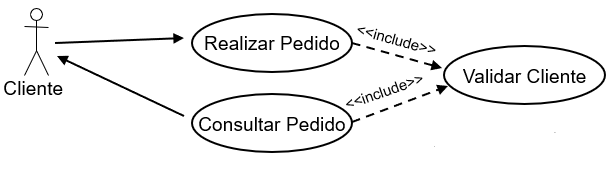
\includegraphics[width=0.9\textwidth]{Imagenes/IncludeCasoDeUso.png}
    \caption{Ejemplo con <<Include>>}
\end{figure}

\subsection{Caso de uso: Actor temporal}
Indica el paso del tiempo, tiene una flecha punteada hacia el caso de uso. \textit{Ej. Mensualmente, Diariamente, Semanalmente, Cada X tiempo}

\begin{figure}[!htb]
    \centering
    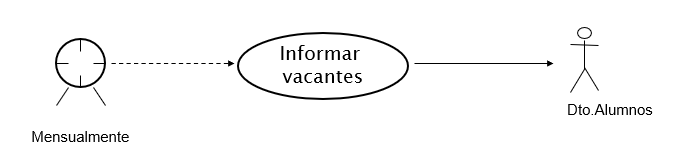
\includegraphics[width=0.9 \textwidth]{Imagenes/ActorTemporalCasoDeUso.png}
    \caption{Un actor temporal: Mensualmente}
\end{figure}

\subsection{Caso de uso: Relaciones de especialización/generalización}
Son actores que pueden tener una flecha hacia otro actor, para indicar que puede iniciar los casos de uso de ese otro actor.

\subsection{Proceso de desarrollo iterativo e incremental}\label{sec:procesoIterativoIncremental}
Voy realizando pequeñas partes del proyecto total. En cada iteración se van capturando requerimientos, análisis, diseño, construcción, testeo y despliegue. Es un mini ciclo de cascada. Cada iteración dura entre 2 y 6 semanas, esto permite que el usuario este probando mucho antes en comparación a cascada (interacción con el usuario constante). Ante cualquier error que ocurra, se esta a tiempo de arreglarlo.

\subsection{Casos de Uso 2.0}
Un slice es una porción de un caso de uso. Estos son hechos durante cada iteración del desarrollo iterativo e incremental.

Busca partir los casos de uso en porciones mas pequeñas, para que sean mas implementables en el lapso de 2 a 6 semanas. Proporciona mucha versatilidad.

\subsection{Historias de usuario}
Las historias de usuario son descripciones breves y simples de una funcionalidad, escritas desde la perspectiva que necesita una determinada capacidad del sistema. \textit{Ej. Usuario, área de negocio, o cliente}

\subsubsection*{Componentes}
\begin{itemize}
    \item ID
    \item Titulo: Texto descriptivo de la historia
    \item Descripción: Como [rol], quiero [objetivo], para poder [beneficio]
    \item Estimación: Cuanto va a llevar implementarla (conocida también como puntos de historia)
    \item Valor: valor numérico que aporta importancia a la historia, generalmente de 1 a 5. El objetivo es maximizar el valor y la satisfacción percibida por el cliente o usuario en cada iteración.
    \item Dependencias: Procurar que no existe dependencia entre historias, los que no sea posible indicarla.
    \item Pruebas de integración: Clarifican el contexto en que ocurre la historia, y facilitan saber cuando están terminadas las historias.
\end{itemize}

Ej. 
\begin{itemize}
    \item COMO usuario QUIERO poder acceder al catalogo de cursos PARA poder tomar decisiones de los cursos en los cuales inscribirme.
    \item COMO usuario QUIERO poder buscar transacciones PARA poder detectar gastos innecesarios en mi cuenta durante cierto periodo de tiempo.
\end{itemize}

\begin{figure}[!htb]
    \centering
    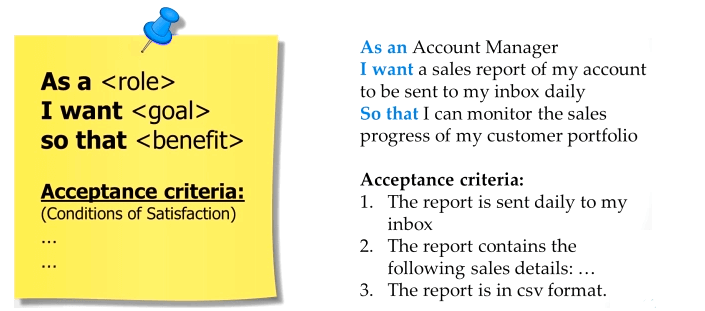
\includegraphics[width=0.9\textwidth]{Imagenes/UserStory.png}
    \caption{Modelo de una historia de usuario}
\end{figure}


\subsubsection*{Buenas practicas}
\begin{itemize}
    \item Deben mapear a \textbf{una sola} funcionalidad del producto, software.
    \item Es una buena practica usar personajes en vez de roles. \textit{Ej. Alumno en vez de usuario}.
    \item Se hacen en fichas.
\end{itemize}

\subsubsection*{INVEST}
Es un metodo para escribir buenas historias de usuario.
\begin{itemize}
    \item Independiente: No deben depender unas de otras, si ocurre tratar de dividir o combinar.
    \item Negociable: Deben ser negociables sus detalles entre cliente/usuario en la <<conversación>>.
    \item Valor: Tiene que ser valiosa para el cliente.
    \item Estimable: Debe ser estimada con la precisión suficiente para ayudar al cliente o usuario a priorizar y planificar su implementación.
    \item Pequeña (Small): Como máximo una iteración.
    \item Testeable: Deben poder probarse y saber que la historia se completo con éxito.
\end{itemize}

\subsubsection*{Criterios de aceptación}
Son una serie de preceptos que validan la implementación de la historia de usuario.
\begin{itemize}
    \item Ayudan al desarrollador a implementarla de forma correcta.
    \item Se pueden mapear sobre los tests de funcionalidades.
    \item Ayudan a QA para dar el OK a la historia.
    \item Definen junto a la descripción la funcionalidad a implementar.
    \item Tienen solo 2 resultados: ÉXITO o FRACASO.
    \item Deben ser interpretados de una única manera por N personas, no deben ser ambiguos.
    \item Deben ser verificables por el cliente rápidamente.
    \item Tienen que ser completos, el grupo debe incluir todas las funcionalidades.
\end{itemize}

Ej.
\begin{itemize}
    \item El nombre de usuario DEBE tener un valor, en caso contrario se mostrara el mensaje de error pertinente.
    \item Si el usuario y la contraseña son correctos, el usuario podrá acceder a la aplicación.
\end{itemize}

\subsubsection*{Conversaciones}
En el mundo ideal los clientes tienen una idea muy clara de lo que quieren desde el principio, y nos lo cuentan con lujo de detalles sin dejarlo en el tintero. En la realidad esto no pasa.

Una historia de usuario abrirá normalmente una conversación entre el equipo de desarrollo y el cliente. Las historias de usuario no cambian a nivel conceptual, son las conversaciones las que las volverán mas detalladas.


\section*{Quinta clase}

\section{Modelo Conceptual}
Dentro de los modelos de requerimientos.

\subsection{Diagramas de clases conceptuales}
Las clases representan los bloques de construcción mas importantes de cualquier sistema.

\begin{itemize}
    \item Nombre
    \item Atributos: propiedades del elemento que estamos modelando
    \item Operaciones (Métodos): implementación de un servicio
    \item Responsabilidades: lo que le corresponde realizar a la clase,las obligaciones que deben realizar las clases para cumplir con los requerimientos. \textit{Ej. determinar el riesgo de un pedido de un cliente - manejar criterios de fraude específicos del cliente}
\end{itemize}

\begin{figure}[!htb]
    \centering
    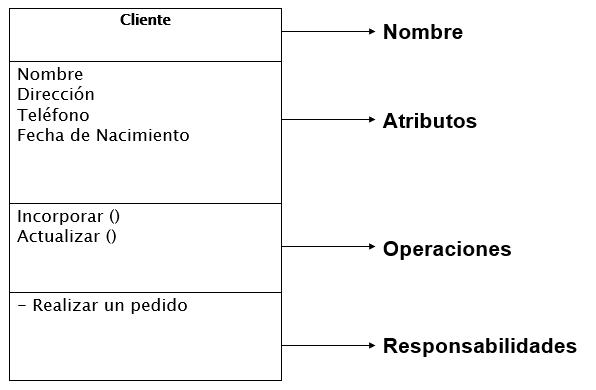
\includegraphics[width=0.9\textwidth]{Imagenes/Clase.png}
    \caption{Modelo de una clase para el diagrama.}
\end{figure}

Es buena practica iniciar el modelaje especificando las responsabilidades, dejando para después los atributos y operaciones. Deben de contener al menos 'una' responsabilidad. (tratar de respetar el Single Responsability Principle)

\subsubsection*{Tipos de clase: MVC}
\begin{itemize}
    \item Las clases conceptuales (de entidad), son las necesarias para cumplir con las responsabilidades asignadas al sistema.
    \item Clase de entorno, maneja el dialogo entre el sistema y el medio externo. Modelan las interfaces del sistema.
    \item Clases de control, coordinan los eventos necesarios para realizar el comportamiento especificado en un caso de uso (Representan su dinámica).
\end{itemize}


\subsubsection*{Identificación}

Para identificar clases, se puede usar la regla practica, usar sustantivos o frases sustantivas que describen responsabilidades del sistema. La otra forma es con tarjetas CRC (Colaboration Responsability Card), que es una técnica de modelado para refinamiento de clases.

De acá se tiene una lista inicial de clases, y con esto se hace un diagrama de clases participantes (sin colaboraciones).

\subsubsection*{Relaciones entre clases}
\begin{itemize}
    \item De asociación, es entre instancias que se encuentran en un mismo nivel. Tiene nombre de asociación, rol, multiplicidad. Existen la simple, de agregación, de composición y clase de asociación
    
    \begin{itemize}
        \item Simple, relación de asociación entre objetos de una clase. \textit{Ej, Nombre de asociación: Emplea} Recta que une las dos clases. El rol puede omitirse si es trivial. La multiplicidad es obligatoria.
        \item Agregación, se tiene una clase que representa un todo, y otra una parte. Si se elimina una instancia del todo, las partes siguen existiendo. Tiene un rombo vacío del lado del todo.
        \item Composición, fuerte relación de pertenencia y vida entre un todo y las partes. Si se elimina e todo, las partes asociadas mueren. Rombo negro del lado del todo. Un todo puede tener muchas partes, pero no puede haber una parte de muchos todos.
        \item Clase de asociación, es una nueva clase que surge de la asociación de dos clases, contiene elementos que no le son propios a las clases relacionadas. Existen una sola vez, si se repite se convierte asociación simple.
    \end{itemize}
    
    \item De generalización, especialización: Es una relación que conecta una clase general con una mas especializada. (Subclase) La clase hijo siempre es instanciable, la padre puede o no serlo. Si no lo es, se dice abstracta. el discriminador indica en base a que especializo.
    
    \item De uso, dependencia, conoce a determinada clase ya que la usa en algún momento, puede ser porque se la pasan por parámetro. No guarda una referencia a ese objeto.
    \item De realización, indica la implementación de interfaces.
\end{itemize}

\begin{figure}[!htb]
    \centering
    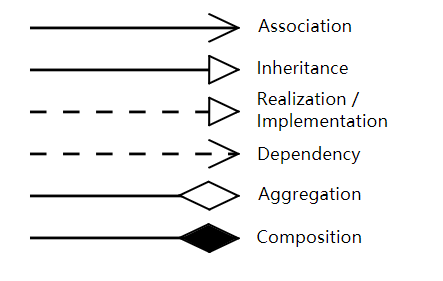
\includegraphics[width=0.5\textwidth]{Imagenes/ClassDiagramArrowTypes.png}
    \caption{Los tipos de flechas}
\end{figure}

\begin{figure}[!htb]
    \centering
    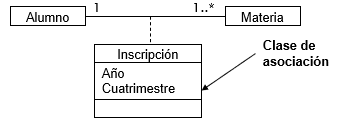
\includegraphics[width=0.5\textwidth]{Imagenes/ClaseDeAsociacion.png}
    \caption{Ejemplo de una clase de asociación.}
\end{figure}


\newpage

\section*{Sexta clase}
\section{Diagramas de interacción entre objetos}
La interacción entre objetos comprende el conjunto de mensajes que son intercambiados entre objetos.

Estos diagramas describen la manera en que colaboran grupos de objetos para cierto comportamiento. Se usan cuando se quiere ver el comportamiento en un escenario predefinido.

Ambos tipos de diagramas son equivalentes. De cada uno puedo llegar al otro. Se enumeran los mensajes en ambos.

\subsection{Diagrama de secuencia}
Muestran el orden temporal de los mensajes y el paso de mensajes. 'Perspectiva cronológica de las interacciones'.

\begin{figure}[!htb]
    \centering
    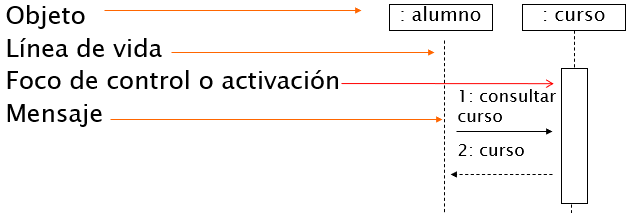
\includegraphics[width=0.9\textwidth]{Imagenes/DiagramaDeSecuencia.png}
    \caption{Elementos de un diagrama de secuencia}
\end{figure}

\subsection{Diagrama de colaboración}
Muestra la organización estructural de los objetos que envían y reciben mensajes. 'Perspectiva espacial de las interacciones'

Linea entre objetos que intercambian mensajes y otra linea indicando la dirección.

\begin{figure}[!htb]
    \centering
    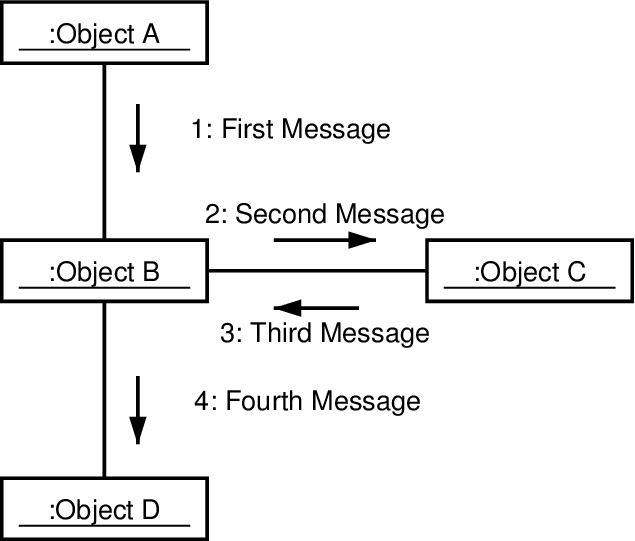
\includegraphics[width=0.5\textwidth]{Imagenes/CollaborationDiagram.png}
    \caption{Modelo de un diagrama de colaboración}
\end{figure}

\newpage

\section*{Séptima clase}
\section{Modelo de Estado de Objetos}
Esta dentro de los modelos de requerimientos.

\subsection{Estado}
Es una condición o una situación en la vida de un objeto durante la cual satisface una condición, realiza alguna actividad o espera algún evento.

Tienen varias partes: nombre, transiciones, condiciones de transición, acciones, transiciones temporizadas, sub-estados, super-estados.

\subsection{Diagrama de estados}
Muestra los cambios de estado existentes en un objeto durante su ciclo de vida. Muestra el comportamiento que especifica las secuencias de estados por las que pasa un objeto. También muestran como se reflejan los cambios que se producen.

Estos diagramas son grafos dirigidos, tienen un estado inicial y final (pueden ser varios estados finales) diferenciados del resto. La transición entre estados es instantánea y se debe a la ocurrencia de un evento. (La definición de autómata básicamente.)

\begin{figure}[!htb]
    \centering
    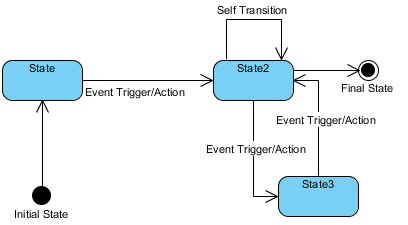
\includegraphics[width=0.8\textwidth]{Imagenes/StateDiagram.png}
    \caption{Diagrama de estados generico}
\end{figure}

Describe el comportamiento de un objeto a través de varios casos de uso. Es útil combinarlo con otros diagramas, \textit{Ej. Diagramas de secuencia}.

\begin{itemize}
    \item Acciones: es la solicitud de un servicio a otro objeto. \textit{Ej. Evento[condición]/Acción - La acción podría ser otroObjeto.operacion()} Pueden tener palabras claves, Entry como una acción a ejecutar al ingresar al estado, un Exit como operación al salir, y un Do que es una acción a realizar mientras esta en el estado. Estas palabras clave están dentro del grafo, el estado. Pueden tener mas de uno.
    \item Transiciones Temporizada: indican un tiempo para el cambio de estado si no ocurre el evento que debía de ocurrir \textit{Ej. "después de 30 segundos", puede ir si se anula una transacción porque no se pago}.
    \item Relaciones de Jerarquía - Superestados - Subestados: Buscan reducir la complejidad de los diagramas generalizando los estados. la entrada puede hacia estas generalizaciones puede ir a los estados específicos con una flecha directo, o un nuevo circulo indicando el comienzo (es preferible el circulo para que no se sepa desde los niveles superiores.).
\end{itemize}

\begin{figure}[!htb]
    \centering
    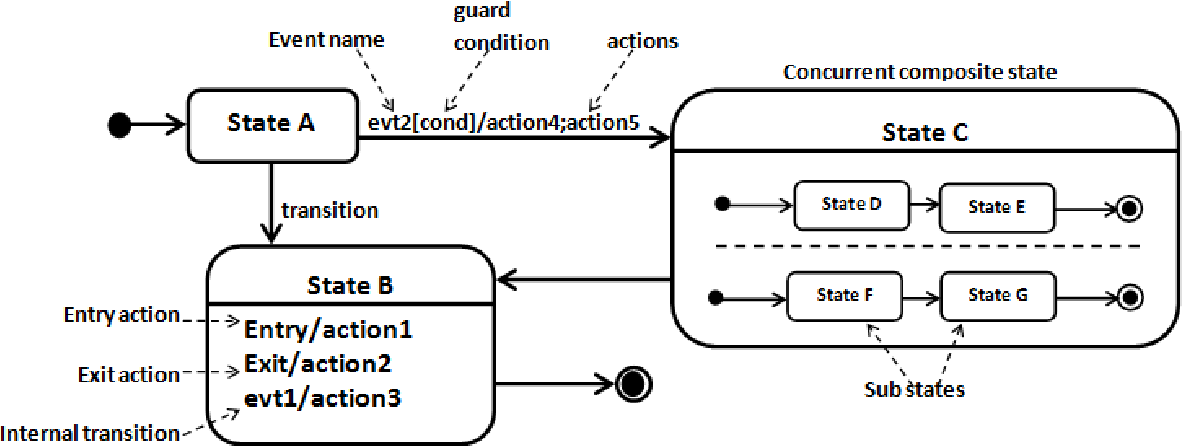
\includegraphics[width=0.8\textwidth]{Imagenes/StateDiagramWithActions.png}
    \caption{Diagrama de estados con acciones en State B}
\end{figure}

Antes de hacer el diagrama hay que contextualizar sobre el objeto al que le vamos a hacer el diagrama.

\begin{figure}[!htb]
    \centering
    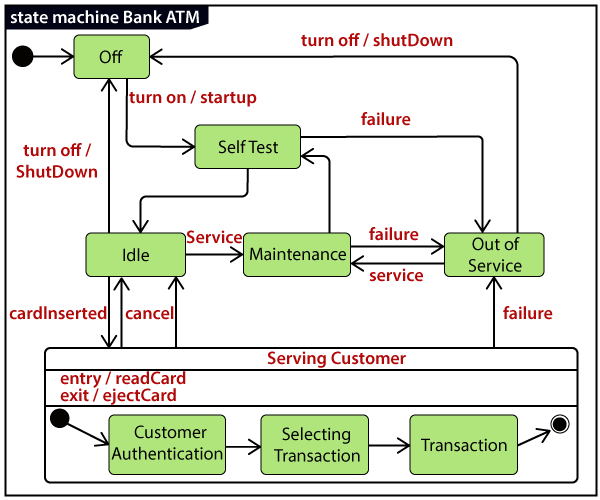
\includegraphics[width=0.8\textwidth]{Imagenes/StateDiagramExample.png}
    \caption{Ejemplo de un diagrama de estados}
\end{figure}

%%%%% Storytelling
% Mas ludico
% Orientado a una narrativa
% Es el arte de contar historias, recreamos historias para poner en contexto y comunicar las necesidades de nuestros usuarios o beneficiarios de los resultados de nuestro sistema
% Se busca generar una conexion con una persona, para ver si entendimos las necesidades.
% Lenguaje sensorial para persuadir al publico.
% Tecnica: Tiene que tener historia, contenida, experiencia/s, ser creativa. Marketing, emocion, compartible, comunicable.
% Estructura basica: Tema - Argumento: con una cronologia como van sucediendo las cosas - Trama: como articulo los hechos en esta historia, la estructura que va a tener - Sentido: para que la voy a contar, por que la transmito
% 2 componentes: Tiene una parte racional (de los hechos), tangible. Se mezcla con la parte sentimental (mezclar con la parte mas humana y sentimental)
% Tecnica narrada y oral. En el TP la reforzamos con la tecnica Visual Thinking.
% Visual Thinging: Mientras voy narrando (storytelling) voy haciendo graficos. 
% Facilitacion Grafica: dibujos sencillos y basicos para que los conceptos se entiendan y comprendan mas facil.
%%% Ejemplo
% 

\section*{Octava y novena clase}
\section{Lean UX}
Es 'dar luz a la verdadera naturaleza de nuestro trabajo y con \emph{menos enfasis en los entregables} y con mayor foco en la experiencia que esta siendo diseñada (la solucion)'.

Se remonta al método Lean Startup
\subsection{Lean Startup}
Tiene cinco postulados.
\begin{enumerate}
    \item Hay emprendedores en todos lados.
    \item Emprender es administrar. (En su sentido mas amplio)
    \item Generar conocimiento valido.
    \item Innovación medible. (Si no podemos medir, no podemos controlar el éxito del proyecto)
    \item Proceso Build-Measure-Learn (Construir-Medir-Aprender).
\end{enumerate}

\subsection{Lean UX vs Diseño Centrado en el Usuario (DCU)}

\begin{center}
\begin{table}[!htb]
\centering
\begin{tabular}{|l|l|}
\hline
\rowcolor[HTML]{FFFE65} 
\multicolumn{1}{|c|}{\cellcolor[HTML]{FFFE65}Lean UX} & \multicolumn{1}{c|}{\cellcolor[HTML]{FFFE65}DCU} \\ \hline
Generar Conocimiento Validado                         & Hacer pruebas con usuarios                       \\ \hline
Innovacion Medible                                    & Tomar metricas                                   \\ \hline
Pivotear                                              & Iterar                                           \\ \hline
MVP(Minium Viable Product)                            & Prototipado iterativo                            \\ \hline
Costumer Development                                  & Trabajo de campo                                 \\ \hline
\end{tabular}
\end{table}
\end{center}

\newpage

\subsection{Build-Measure-Learn}
Es un ciclo iterativo en el cual se parte de determinadas ideas, se construye rapidamente (code faster) un prototipo, se hacen mediciones (measure faster), y con estas mediciones se puede aprender (learn faster). Una vez completada la vuelta se repite.

\begin{figure}[!htb]
    \centering
    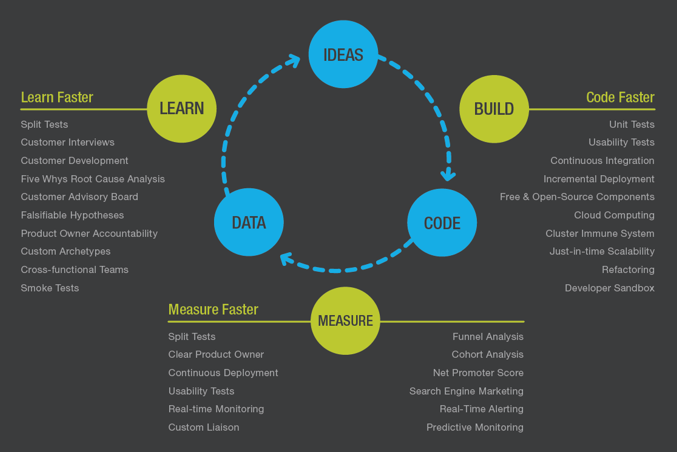
\includegraphics[width=0.9\textwidth]{Imagenes/Build-Measure-Learn.png}
    \caption{Ciclo que se sigue}
\end{figure}

\subsection*{Consideraciones al emprender un proyecto}

\begin{itemize}
    \item Hay que saber distinguir entre lo que quiere el emprendedor y lo que quieren los usuarios.
    \item Los emprendedores son los padres de la 'criatura'. La capacidad de juicio critico esta sesgado. El que tiene que opinar del producto son los usuarios, tienen que dar el juicio.
    \item Las personas 'dicen' es diferente a lo que las personas 'hacen'. (Tenerlo en cuenta cuando se hacen las pruebas, se mejora cuando se tiene en cuenta lo que hacen) (Observar las conductas de las personas) \textit{Ej. Focus Group}
    \item La capacidad de 'resiliencia' de los emprendedores, muy necesaria. Se necesita una alta capacidad de 'resiliencia'.
    \item Hay que poder medir el 'valor' que perciben los clientes a nuestro producto. No es agregar \emph{features} al producto continuamente si es que los clientes no lo perciben.
    \item Hay que poder identificar 'quienes' van a ser nuestros futuros usuarios.
    \item Siempre se va a tener un alto grado de incertidumbre.
    \item Nosotros como emprendedores, no somos los usuarios pero decidimos como si lo fuéramos, esto se debe de evitar. 
\end{itemize}

\subsection{Declaración de supuestos}
El método Lean UX no comienza con requerimientos, empieza con supuestos. A partir de estos se crean y validan diferentes hipótesis. De estas validaciones se miden los resultados, comparándolos con los esperados.

En el procesos suponemos que el producto a desarrollar esta orientado a personajes (arquetipos de personas).

\subsection{MVP}
Un MVP es un producto mínimo viable que se usa para validar las hipótesis. Esta formado por artefactos que crea el estudio de diseño. Cada etapa de diseño tiene un tiempo estimado de iteración.


\begin{center}
\textit{'Un producto mínimo viable es la versión de un nuevo producto que permite a un equipo obtener la máxima cantidad de aprendizaje validado sobre los clientes, con el menor esfuerzo posible'} - Eric Ries
\end{center}

El objetivo del MVP es obtener aprendizaje y generar valor en el producto. Los MVP se pueden clasificar en prototipos, descripción, y producto con funciones mínimas. La calidad de un MVP incrementa a medida que se van haciendo las iteraciones en el ciclo de vida.

La calidad de los MVP debe ser: \textit{Keep. It. Simple. Stupid.} Fallar rápido y barato, debido a que es una inversión en un prototipo que después puede cambiarse.


Al comenzar la planificación de un MVP hay que pensar:
¿Existe una necesidad por parte de un usuario para la funcionalidad a implementar?
¿Existe valor en la funcionalidad a implementar?
¿Existe usabilidad en la funcionalidad a implementar?


\subsubsection*{Prototipos}
Se presenta a clientes potenciales una simulación del producto con suficiente nivel de detalla para comprender la funcionalidad a validar. 
No es un producto.

\subsubsection*{Descripciones}
Se capta la atención de clientes potenciales con una descripción e información general sobre el producto/servicio. Son los mas baratos y simples. \textit{Landing page, correos, vídeos}

\subsubsection*{Producto}
Es código funcionando, no todo el desarrollo. Es el mas costoso. Solo se realiza la funcionalidad necesaria para validar la hipótesis.

\subsubsection*{A quien se dirige}

\begin{itemize}
    \item Innovator: obtienen el producto recién sale
    \item Early adopters: adoptan el producto de forma temprana
    \item Early majority: 
    \item Late majority
    \item Laggards: La inversa a los innovadores.
\end{itemize}

\begin{figure}[!htb]
    \centering
    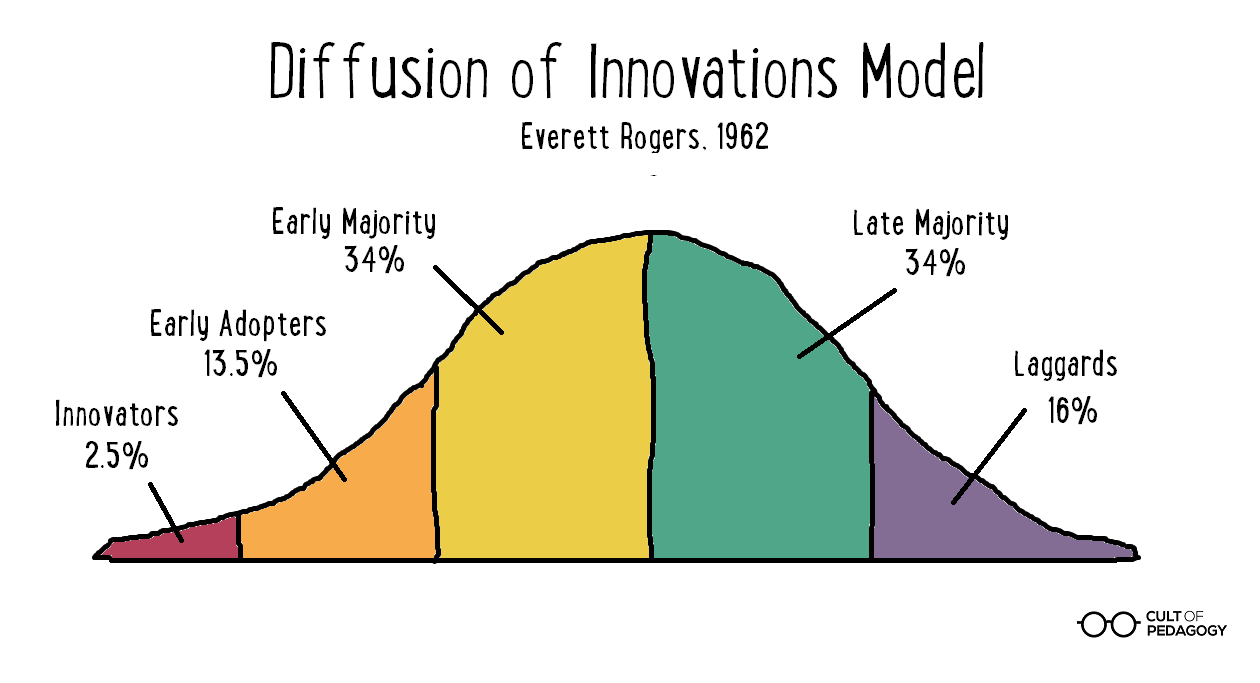
\includegraphics[width=0.8\textwidth]{Imagenes/CurvaInnovacion.png}
    \caption{curva de adopción de la innovación}
\end{figure}

\subsubsection*{Obstáculos al desarrollo}

\begin{itemize}
    \item Tiempo
    \item Alcance
    \item Recursos
    \item Legales, patentes
    \item Miedo a la competencia
    \item Miedo al riesgo
    \item Miedo a la frustración
\end{itemize}

\subsubsection*{Experimento}
Es el comienzo del proceso de validación. Se utiliza para probar el MVP con usuarios, para comprobar las hipótesis.

Se debe mostrar o probar con clientes potenciales. Estos deben utilizar y explorar el prototipo lo mas libremente posible, para obtener mas feedback.

Prueba de estabilidad, identifican problemas de usabilidad en el producto (prototipo). Permite reunir información cuantitativa y cualitativa del desempeño.

Participa el facilitador (conduce la prueba), los observadores (toman notas), el wizard of Oz (simula la interacción en el prototipo si es necesario), y los usuarios (personas con el perfil necesario, protopersonas)

Es necesario definir el perfil del usuario, el contexto de uso, y la meta.

\begin{enumerate}
    \item El facilitador pide comenzar la prueba
    \item El facilitador lee el primer escenario y tarea, el usuario lo inicia
    \item El usuario dice que piensa, facilitador y observador toman notas de lo que dice y hace el usuario
    \item Continua la prueba a través de los escenarios y tareas
    \item Se logra la meta o el tiempo, el facilitador termina la prueba
    \item El facilitador agradece al usuario por su participación
\end{enumerate}

Se evalúa el producto, no al usuario en las pruebas de usabilidad.

Se realiza Lean User Research, se realiza un rápido registro de los aspectos a considerar.
\begin{itemize}
    \item Stoppers: Dudas y problemas que tuvieron los participantes, cuando se quedan trabados
    \item Values:
    \item Feedback: Continuo (calendario permanente de actividades, simplificar el protocolo y entorno de experimentación, simplificar reclutamiento de usuarios, el equipo trabaja todo el tiempo, se reúne el equipo rápidamente luego de la prueba) y colaborativo (todo el equipo trabaja en conjunto sobre la declaración de hipótesis y construcción del MVP)
    \item Recommendations: Sugerencias del moderador desde la perspectiva del usuario para corregir problemas de usabilidad y mejorar la experiencia.
\end{itemize}


\subsubsection*{Herramientas}
\begin{itemize}
    \item Business Model Canvas, gestiona el modelo de negocio
    \item Validation Board, gestiona el ciclo de vida del producto
    \item Scope Canvas, centrado en la información relevante del producto, ver en \ref{sec:ScopeCanvas}.
\end{itemize}

\begin{figure}[!htb]
    \centering
    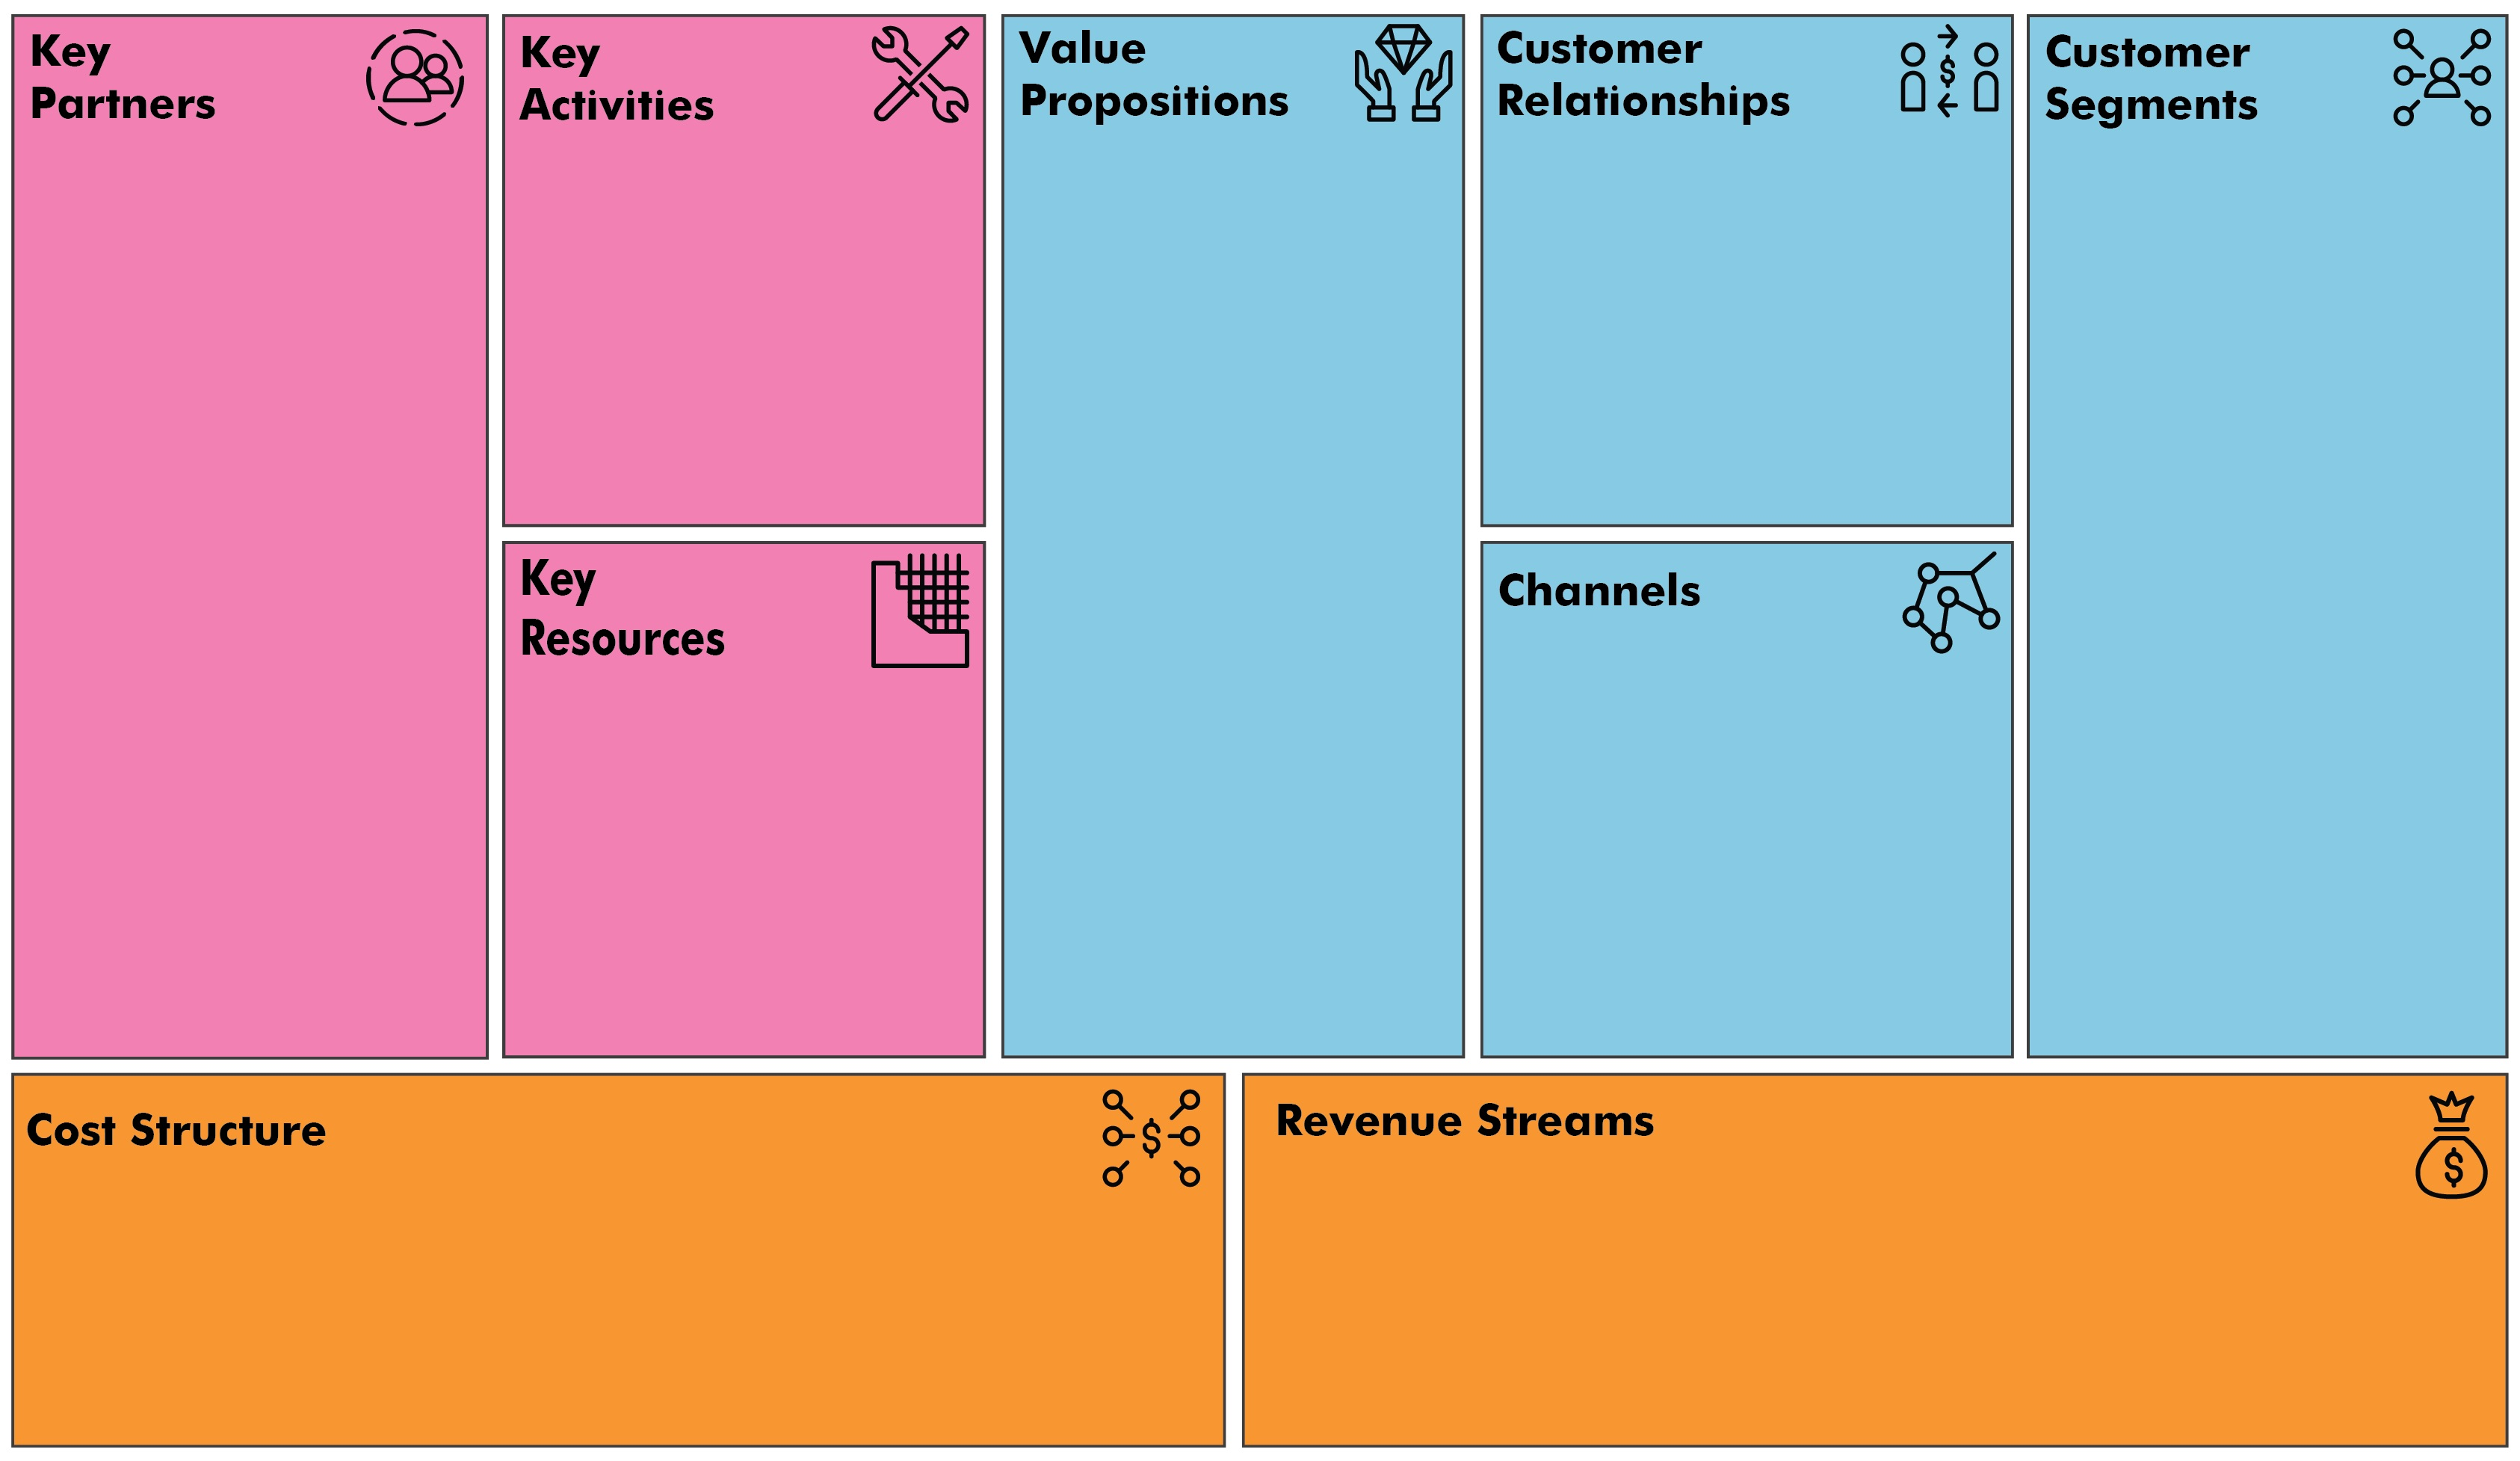
\includegraphics[width=0.8\textwidth]{Imagenes/BusinessModelCanvas.jpg}
    \caption{Plantilla Business Model Canvas}
\end{figure}

\begin{figure}[!htb]
    \centering
    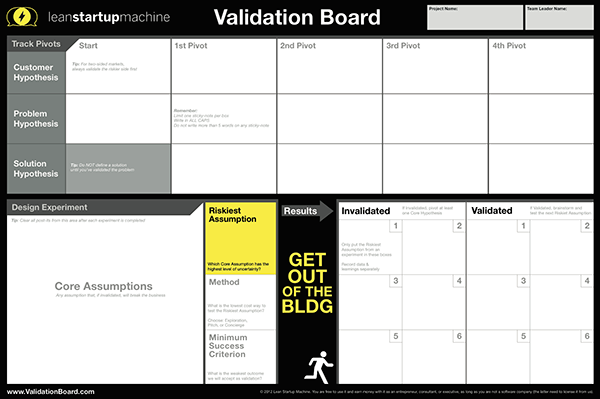
\includegraphics[width=0.8\textwidth]{Imagenes/ValidationBoard.png}
    \caption{Plantilla Validation Board}
\end{figure}

\newpage

\section{Scope Canvas}\label{sec:ScopeCanvas}

El Scope Canvas combina elementos que ya se venían trabajando en proyectos de lean UX de forma separada. Nos permite establecer formas de observar el éxito del proyecto. Es una foto del momento.


El Scope Canvas no nos dice como vamos a trabajar.

\subsection{Plantilla}

\begin{figure}[!htb]
    \centering
    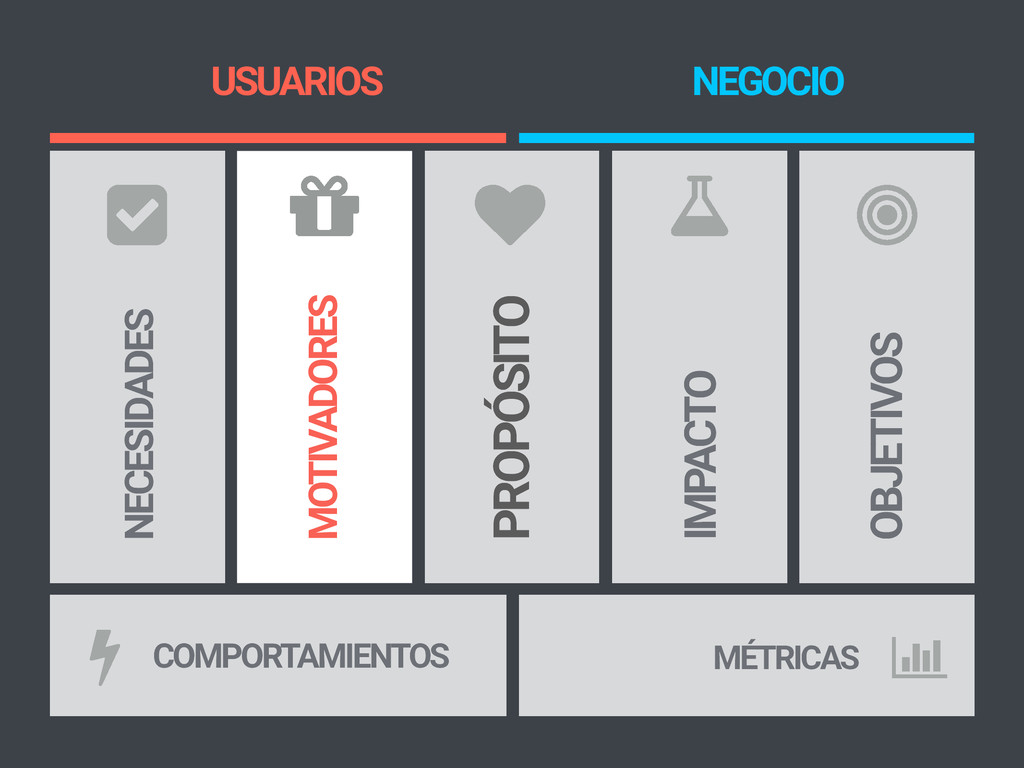
\includegraphics[width=0.7\textwidth]{Imagenes/ScopeCanvas.jpg}
    \caption{Plantilla de Scope Canvas}
\end{figure}



\begin{itemize}
    \item Hay que definir todas las partes que aparecen en la imagen.
    \item Con Scope Canvas se logran equipos de trabajo mas alineados en torno a las metas comunes. Que se tenga una cultura mas explicita.
    \item La visión de los actores clave desde el principio del producto que se esta ideando.
\end{itemize}


\subsubsection*{El propósito}

\begin{itemize}
    \item ¿que hace que esto valga la pena? ¿Por que hacemos esto? ¿Que nos mueve?
    \item Nos mueve hacer esto porque...
    \item El propósito debe servir a la organización y a los usuarios por igual, muy ambicioso y muy estimulante. Hay que ser sincero con las motivaciones personales.
    \item \textit{Ej. Que todos puedan ahorrar energía - Conectar al mundo en un instante - Una sociedad mas respetuosa - Organizar la información del mundo (Google)}
\end{itemize}

\subsubsection*{Necesidades}

\begin{itemize}
    \item Esta en la parte de los usuarios. ¿Que problemas y/u oportunidades insatisfechas tenemos el potencial de atender? 
    \item Nuestros usuarios necesitan/desean...
    \item Puede haber varios segmentos de usuarios. Para proyectos multi-sided se defina al menos una necesidad por cada segmento de usuario o cliente.
    \item Hay que evitar mencionar posibles soluciones al declarar necesidades. (Evitar el ¿Como?)
    \item Los emprendedores deben detectar estas oportunidades. Son valor agregado para los usuarios que ellos aun no visualizan. Para validar las necesidades hay que investigar, crear historias (storytelling), y sintetizar.
    \item \textit{Ej. Sacar su certificado sin ir a las oficinas - Ahorrar energía - Aprender un nuevo idioma}
\end{itemize}

\subsubsection*{Objetivos}

\begin{itemize}
    \item Son del negocio a corto plazo. ¿Cuales son los objetivos del proyecto? ¿Que esperamos obtener? ¿cual es la prioridad?
    \item El objetivo es...
    \item Los objetivos deben ser cuantificables y medibles. No necesariamente hay que determinar uno con numero. Hay que evitar los objetivos vagos (no se pueden medir). Los objetivos deben relacionarse con la adopcion de usuarios, no son solo internos.
    \item En este momento hay que preguntarse como se sustentara el proyecto. Puede ser útil realizar el Buisness Model Canvas antes de llenar esa sección.
    \item \textit{Ej. Reducir el tiempo de compra en un 50\% - Crecer en un 25\% anual}
\end{itemize}

\subsubsection*{Motivadores}

\begin{itemize}
    \item Se tienen motivaciones de mediano y largo plazo. ¿Que mejora entregamos a los usuarios para satisfacer sus necesidades? 
    \item Los usuarios adoptaran el producto si les entregamos...
    \item Las necesidades y los motivadores están relacionados.
    \item Los futuros usuarios ya están intentado satisfacer sus necesidades. Antes de definir los motivadores debemos investigar cuales son las maneras actuales de satisfacer dichas necesidades, y de que forma es mejor nuestra idea.
    \item La innovación debe reflejarse en los motivadores. 
    \item Los motivadores los validamos a través de las acciones. Si el motivador es correcto, los usuarios adoptan el producto realizando acciones.
\end{itemize}

\subsubsection*{Acciones (Comportamiento)}

\begin{itemize}
    \item ¿Que acciones especificas de los usuarios implican conversión? ¿Como sabremos si estamos entregando los motivadores correctos?
    \item Esperamos que los usuarios...
    \item Las acciones tienen que ser cruciales y observables.
    \item \textit{Ej. Comprar- Transportarse en bicicleta en lugar de en auto - Registrarse}
\end{itemize}

\subsubsection*{Impacto}

\begin{itemize}
    \item El impacto es a mediano y largo plazo. ¿cual es el potencial del proyecto si nos va bien? ¿En que esperamos convertirnos si nos va bien?
    \item Nuestras metas de largo plazo son...
    \item Es el impacto en el negocio. Nos permite visualizar el éxito de largo plazo del proyecto. Nos acerca al propósito. Siempre es observable por terceros. tiene un efecto poderoso en la motivación.
    \item No hay que mezclar impactos con objetivos. Impacto es observable, el objetivo es medible.
    \item El impacto debe reflejas un éxito masivo, a gran escala.
    \item Hay que prestar atención a los impactos no esperados y corregirlos.
\end{itemize}

\subsubsection*{Métricas}

\begin{itemize}
    \item ¿Como sabemos que los objetivos se están cumpliendo> ¿Donde medimos? ¿Como medimos?
    \item Mediremos ... para saber si estamos logrando el objetivo
    \item Tienen que estar expresadas en datos. Nos cuentan la historia de como le fue a nuestros usuarios. No hay que engañarse.
    \item Las métricas deben responder a las acciones de los usuarios y a los objetivos que estamos siguiendo.
    \item \textit{Ej. Recurrencia de uso - tiempo para completar una tarea - SUS (system Usability Scale) - NPS (Net Promoter Score)}
\end{itemize}

\subsection{Reglas}
\begin{itemize}
    \item Se usan \textit{post-its} y lapices grandes. Se debe de ser simple y breve. Hay que debatir, no juzgar.
    \item Dura típicamente 2 horas. Máximo 15 personas.
    \item El debate permite simplificar todos los \emph{post-its}.
\end{itemize}

\section*{Décima y Onceava clase}


\section{Desarrollo Iterativo e Incremental}

Procesos de desarrollo de software, es una forma disciplinada de asignar tareas y recursos en un proyecto de software con el objetivo de tener un producto de calidad dentro de plazos y presupuestos predecibles.

Permite comprender de forma creciente los requerimientos a medida que se va haciendo crecer el sistema. Se logra reducir los riesgos del proyecto

Se vio en \ref{sec:procesoIterativoIncremental}.

\section{Manifiesto Ágil}
\subsection{Valores}
Son 4, hay que mirarlos como una balanza, quien tiene mayor peso.
\begin{itemize}
    \item \textit{Valorar: al individuo y las interacciones del equipo de desarrollo sobre el proceso y las herramientas.} La gente es el principal factor de éxito de un proyecto. Significa darle mayor preponderancia a las personas. Sobre los procesos y herramientas no quiere decir de no darles importancia, dice de no ponerlas sobre las personas.
    \item \textit{Desarrollar software que funciona mas que conseguir una buena documentación.} No producir documentos a menos que sean necesarios de forma inmediata para tomar una decisión importante.
    \item \textit{La colaboración con el cliente mas que la negociación de un contrato.} Tiene que haber una interacción constante entre el cliente y el equipo de desarrollo. Llevar al pie de la letra al contrato (con plazos y costos preestablecidos) puede llevar al fracaso.
    \item \textit{Responder a los cambios mas que seguir estrictamente un plan.} La habilidad de responder a los cambios determina el éxito o fracaso del proyecto.
\end{itemize}

\newpage

\subsection{Principios}
Son 12, se derivan de los valores.

\textbf{Principios generales}

\begin{enumerate}

    \item \textit{La prioridad es satisfacer al cliente mediante entregas tempranas y continuas de software que le aporten valor.} Un proceso es ágil si a las pocas semanas de empezar ya estoy entregando software que funcione (aunque sea rudimentario). El cliente decide si pone en marcha el software con la funcionalidad que funciona o no.
    \item \textit{Dar la bienvenida a los cambios.} Deben verse como algo positivo. La estructura debe ser flexible para poder incorporarlos sin demasiado coste.
    
    \textbf{Relativos al Proceso de desarrollo}
    
    \item \textit{Entregar frecuentemente software que funcione desde un par de semanas a un par de meses.} (2 semanas a un mes y medio)
    \item \textit{La gente del negocio y los desarrolladores deben trabajar juntos a lo largo de todo el proyecto.} Necesita ser guiado por el cliente.
    \item \textit{Construir el proyecto en torno a individuos motivados.} La gente es el principal factor de éxito, todo lo demás queda en segundo plano (proceso, entorno, gestión, etc). Los equipos motivados tiene muchísimo mejor desempeño.
    \item \textit{El dialogo cara a cara es el método mas eficiente y efectivo para comunicar información dentro de un equipo de desarrollo.} Los miembros de equipo deben hablar entre ellos, la principal forma de comunicación.
    \item \textit{El software que funciona es la medida principal de progreso.} Se mide en el estado por el código generado que este funcional. \textit{Proyecto en 50\% si el 50\% de los requisitos esta cubierto}
    \item \textit{Los procesos ágiles promueven un desarrollo sostenible en el tiempo.} No se trata de desarrollar lo mas rápido posible, si no de mantener el ritmo durante la duración del proyecto, asegurando que la calidad de lo producido es máxima.
    
    \textbf{Relativos al Equipo de desarrollo}
   
    
    \item \textit{La atención continua a la calidad técnica y al buen diseño mejora la agilidad.}
    
    \item \textit{La simplicidad es esencial.}
    \item \textit{Las mejores arquitecturas, requisitos y diseños surgen de los equipos organizados por si mismos.} Todo el equipo es informado de las responsabilidades, estas recaen sobre todos sus miembros. El propio equipo decide la forma de organizarse.
    \item \textit{En intervalos regulares, el equipo reflexiona respecto a como llegar a ser mas efectivo, y según esto ajusta su comportamiento.}
\end{enumerate}

\newpage

\section{SCRUM}
Es un proceso iterativo e incremental utilizado para la construcción de productos de Software. Se compone de iteraciones llamadas Sprints, estas son fijas en el tiempo. Se recomienda una duración de 1 a 4 semanas. El objetivo de las Sprints es construir un incremento del producto que potencialmente pueda ser usado por los clientes. No nos serviría algo que no pudiéramos utilizar al final de la iteración.

\begin{figure}[!htb]
    \centering
    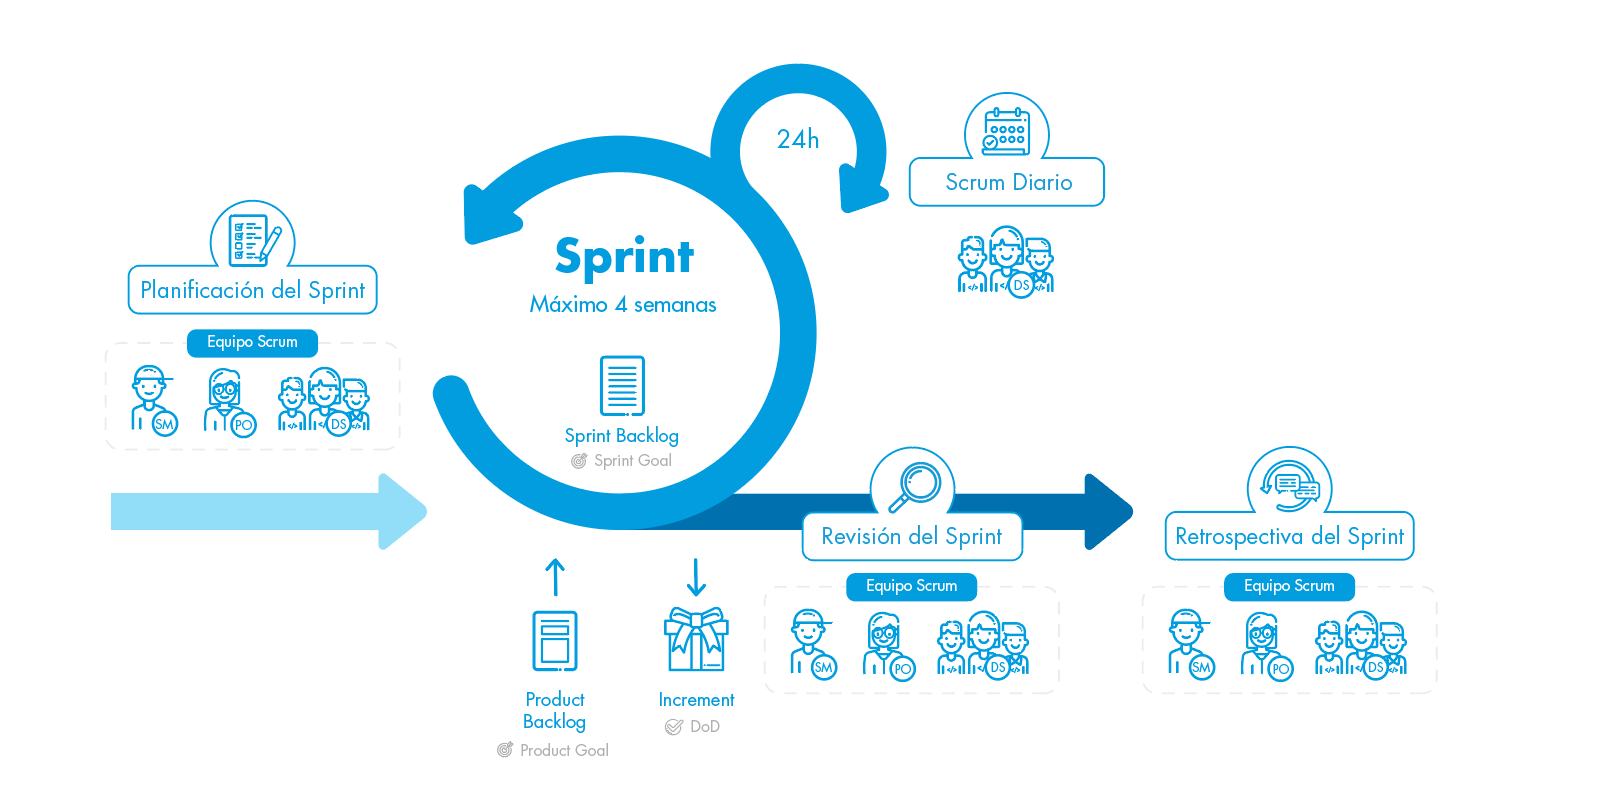
\includegraphics[width=0.9\textwidth]{Imagenes/Scrum.png}
    \caption{Proceso Scrum}
\end{figure}

\subsection{Artefactos}

\subsubsection*{Pila de producto}
Una vez que tengamos claro que personas son a las que vamos a aportar valor, es necesario recopilar en un único sitio todas las ideas, funcionalidades y elementos que van a componer el producto. Estos van ordenados por valor de negocio (arriba los que aportan mas). Esto se llama Pila de Producto o Product Backlog. Los elementos se conocen como PBIs (Product Backlog Items), estos contienen como mínimo una descripción, la prioridad que tengan, la estimación en tiempo y costo, y el valor que aporta. Los PBIs podrían ser historias de usuario.

Las características de las pilas de producto deben de ser DEEP (Detallado, estimado, emergente, priorizado)
\begin{itemize}
    \item Detallado: los PBIs próximos (arriba de la pila) deben de tener el mayor detalle.
    \item Estimado: Cada uno nos tiene que servir para planificar, mas arriba, estimaciones mas precisas.
    \item Emergente: Una pila de producto no es estática, va cambiando con el tiempo, se agregan/eliminan elementos.
    \item Priorizado: Mas importantes mas arriba de la pila, menos importantes abajo. Para priorizar hay distintos métodos. \textit{Ej. Método MoSCoW\footnote{M:must have - S:should have - C:could have - W:won't have}
    , Método Kano, Método ROI}.
\end{itemize}

\subsubsection*{PBIs}
Contienen como mínimo una descripción, la prioridad que tengan, la estimación en tiempo y costo, y el valor que aporta. Los PBIs podrían ser historias de usuario (Regla 3Cs - Card - Conversation - Confirmation). (mencionados arriba)

\subsubsection*{Pila del Sprint, Sprint Backlog}
El conjunto de PBIs y las tareas se llama Pila del Sprint (seleccionados por el Product Owner como mas importantes). Para llegar acá de la pila de producto, se hace una reunión de planificación.

Se tiene Pendiente, En progreso, y Terminado. Las tareas mas arriba tienen mayor valor.

\begin{figure}[!htb]
    \centering
    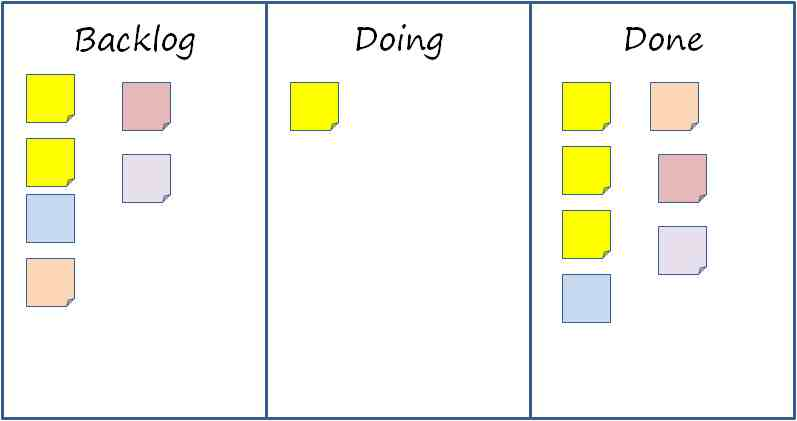
\includegraphics[width=0.8\textwidth]{Imagenes/SprintBacklog.jpg}
    \caption{Sprint Backlog}
\end{figure}

\subsubsection*{Incremento del producto}
Es el resultado de cada Sprint. Buscan que potencialmente se pueda poner en Producción, aportar valor al cliente.

\subsection{Roles}
\subsubsection*{Product Owner}
Para gestionar toda esta comunicación y gestionar la pila de producto existe un rol especifico llamado Dueño de producto (Product Owner), es el responsable de mantener la visión del producto que se va a construir. Tiene que maximizar el valor entregado al final de la Sprint. Asiste a las reuniones de planificación y revisión (DEMO) del Sprint con el equipo de planificación para transmitir la visión del producto.

\subsubsection*{Scrum Master}
Facilita todas las reuniones que se realicen, acompaña al equipo a resolver las problemáticas que aparezcan en el desarrollo. Es el vigía del proceso, vela para que se lleve a cabo sin olvidar que esta pendiente de las personas que conforman el equipo. Debe de tener una buena visión de la organización, buena comunicación y gestión, ser un líder.

\subsubsection*{Clientes, Stakeholders}
Para empezar a construir un producto, antes debe haber una idea o necesidad. Las personas a las que construimos el producto se les llama Interesados o Stakeholders. Hay que saber distinguir a un usuario (cualquiera que use la aplicación) de los clientes (los que pagan por la aplicación).

\subsubsection*{Equipo de Construcción}
El equipo de construcción es el encargado de la construcción del producto en cada sprint. El equipo debe estar enfocado sobre una parte pequeña del producto. Esta formado por todas las personas que desarrollan, desarrolladores, diseñadores, arquitectos, testers, etc. El equipo es multidisciplinario (entre todos puedan dar servicio al proyecto), tienen que poder auto-organizarse (asignar tareas y estimarlas).

El equipo no debe ser de mas de 9 personas.

\subsection{Reuniones}
El Sprint conviene que tenga una duración fija, busca un ritmo sostenido.

\subsubsection*{De planificación}
La primer reunión se llama Reunión de Planificación o Sprint Planning, se selecciona de los PBIs los mas importantes como el desgranado de estos tareas técnicas. Acuden el dueño de producto, el equipo de construcción, el Scrum Master. El resultado es la Pila del Sprint.

El Product Owner explica al equipo de construcción la funcionalidad a construir.


\subsubsection*{Daily}
La Daily, para realizar una gestión de riesgos adecuada y fomentar la comunicación y sincronización entre los miembros del equipo. Se busca detectas problemas e impedimentos que afecten al desarrollo del Sprint. Es una reunión corta de no mas de 15 minutos. Se realiza todos los días. Busca delinear el plan para el día.

\subsubsection*{De revisión, Demo}
Al finalizar el Sprint, se realiza la Reunión de Revisión (Demo) donde se inspecciona todo lo realizado por el equipo de construcción. Acuden el Product Owner, el equipo de construcción y el Scrum Master. Puede ir cualquier persona que quiera ver lo entregado.

\subsubsection*{De retrospectiva, Retro}
Después de la Demo, el equipo se reúne para inspeccionar el proceso y la forma en que trabajaron. El objetivo es detectar posibles problemas y dar soluciones (Foco en las personas y proceso). Se llama Retro. Acuden todos los miembros del equipo de construcción, el Scrum Master y el dueño del producto. La Retro la facilita el Scrum Master

Se pone el foco en las personas y el proceso dejando de lado el producto, acuden todos los miembros del proyecto.
 
\subsubsection*{De refinamiento}
Existe otra reunión cuyo objetivo es trabajar sobre los elementos futuros que entraran en el Sprint. Se llama reunión de refinamiento, se realiza cuando lo decide el equipo SCRUM. Busca añadir detalle, estimaciones y orden a los PBIs.



\subsection{Tablero Kanban}

\begin{figure}[!htb]
    \centering
    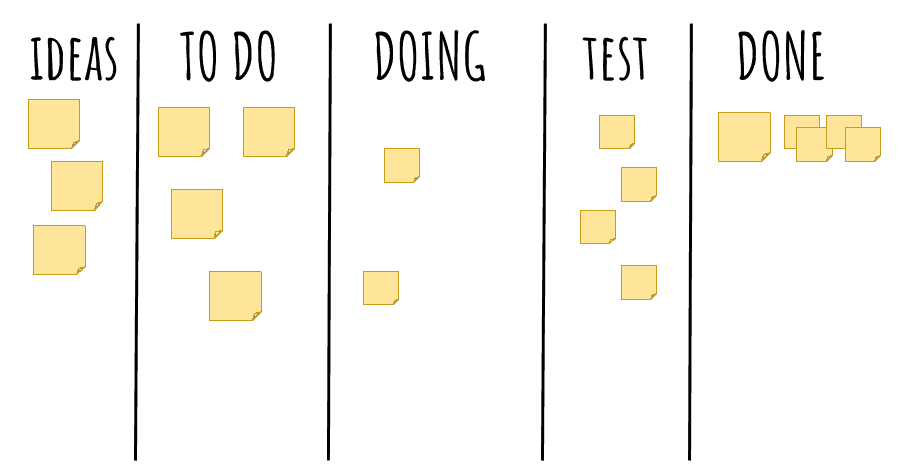
\includegraphics[width=0.8\textwidth]{Imagenes/Kanbanboard.png}
    \caption{Tablero Kanban}
\end{figure}

Se enfoca en la entrega de servicios de una organización, una o mas personas colaboran para la entrega.

\section*{Doceava clase}
\section{Proceso de Desarrollo Unificado - RUP}

Es una forma disciplinada de asignar tareas y responsabilidades en un proyecto de desarrollo de software, con el objetivo de obtener un producto de calidad. RUP (Rational Unified Process), no es un sistema con pasos firmemente establecidos, sino un conjunto de metodologías adaptables al contexto y necesidades de cada organización. Divide el proceso de desarrollo en ciclos, teniendo un producto al final de cada ciclo.

\subsection*{Mejores practicas}
\begin{itemize}
    \item Desarrollo iterativo e incremental del software, lo visto en las secciones anteriores. (N iteraciones, cada una con su mini-ciclo en cascada) en las primeras iteraciones hay mas esfuerzo en captura de requerimientos y modelo de negocio, a medida que se avanza en el proyecto el tiempo se dedica mas a producción, testeo y despliegue. 
    \item Proceso dirigido por casos de uso - RUP contribuye a obtener, organizar, documentar, rastrear, captar y comunicar los requerimientos. Los casos de uso probaron que son una buena forma de obtener los requisitos. Los casos de uso se integrarían a lo largo de todo el proceso.
    \item Uso de arquitecturas basadas en componentes (reusabilidad) - Se basa en poder diseñar tempranamente una arquitectura base ejecutable, esta debe de ser flexible, fácil de modificar, intuitivamente comprensible, y promover la reusabilidad.
    \item Trabajar con modelos visuales (UML)
    \item Verificar la calidad del software - RUP ayuda a planificar, diseñar, implementar, ejecutar y evaluar pruebas que verifiquen las cualidades. Esto tiene que ser parte del proceso de desarrollo, no de un grupo independiente.
    \item Control de cambios - RUP indica como controlar, rastrear y monitorear los cambios dentro del proceso iterativo de desarrollo. Ante un cambio se evalúa la relación costo/beneficio de introducirlo en la versión actual.
\end{itemize}

\begin{figure}[!htb]
    \centering
    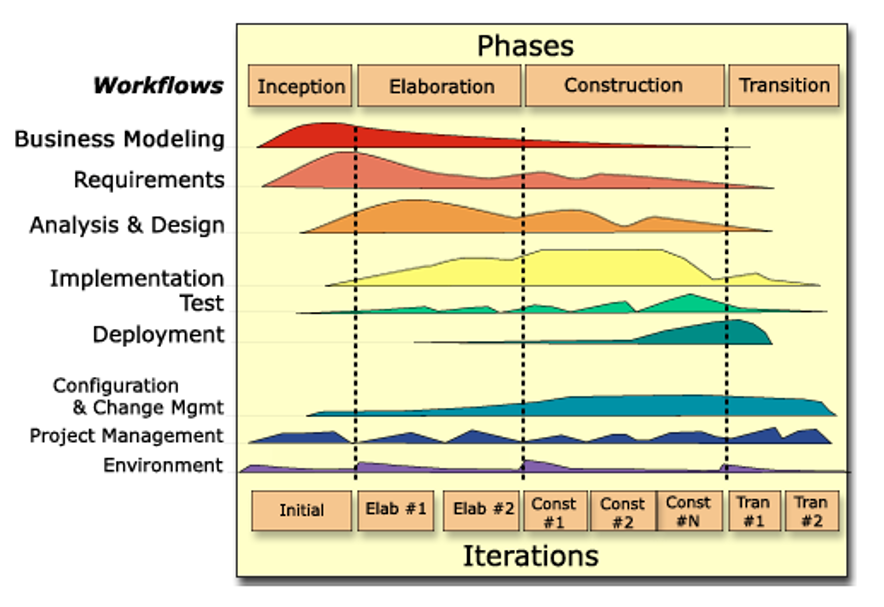
\includegraphics[width=0.7\textwidth]{Imagenes/DistribucionTiempoDesarrollo.PNG}
    \caption{Distribución del tiempo en las fases.}
\end{figure}

\subsection*{Fases de RUP}
Cada ciclo tiene estas fases.

\begin{enumerate}
    \item Inicio (o concepción): Se define el ámbito y los objetivos del proyecto. Se definen las funcionalidades y se identifican las entidades externas con las que se trata.
    \item Elaboración: Busca una arquitectura del sistema estable (el hito). El dominio del problema busca finalizar los casos de uso. Tanto la funcionalidad como el dominio del problema se estudian en profundidad.
    \item Construcción: Busca tener el producto beta (capacidad operacional inicial - hito). Se tiene el producto de software integrado y corriendo en la plataforma adecuada. Se pone mucho énfasis en la producción eficiente.
    \item Transición: Es la release del producto, busca pasar el software desarrollado a la comunidad de usuarios. Hay que tener autosuficiencia por parte de los usuarios.
\end{enumerate}

\subsection*{Componentes del proceso}
\begin{itemize}
    \item Buissness modeling
    \item Requirements
    \item Analysis \& design
    \item Implementation
    \item Test
    \item Deployment
\end{itemize}

\subsection*{Componentes de soporte al proceso}
\begin{itemize}
    \item Environment
    \item Project Managment
    \item Configuration \& change managment
\end{itemize}


\subsection*{Elementos}

\begin{itemize}
    \item Trabajador: Identifica un rol especifico en el proyecto de software. \textit{Ej. diseñador de objetos, de casos de uso, etc}
    \item Actividad: Es una tarea que es responsabilidad de un trabajador. \textit{Ej. Diseñar objetos, Especificar casos de uso}
    \item Artefacto: Resultado parcial o final que es producido y usado durante el proyecto. \textit{Ej. un documento, pruebas, requisitos}
\end{itemize}

\newpage


% graficar/ilustrar lo que quiero mostrar 
% lo que digo, como lo digo - it's a beautiful day and i can't see it
% recitar 'un poema' POEMA
% Prepararse, organizar la forma en que se hara la presentacion, elegir estilo voz y apariencia, manejar nervios y administrar todo armonicamente
% salude y sorprenda a su audiencia
% construir el clima
% ser amigable
% usar el humor
% haga un desafio, preguntas - si nadie responde, 'si nadie se anima, me animo yo...'
% use una cita, cree imagenes verbales
% conocer muy bien el material!!!!, lo que muestro lo tengo que conocer, tengo que saber que es lo que sigue
% aprender sobre la audiencia
% preparar esquemas y notas
% practique con anticipacion, no sale improvisado
% visitar con anticipacion el lugar de la presentacion (especialmente si es formal)
% Organizarse
% Anunciar el tema claramente!!!!!!!!!! Decir que es lo que se va a hablar
% Enunciar el objetivo con anticipacion, hacer un esquema de la presentacion en la introduccion
% Usar transiciones al comienzo de cada seccion principal (verbalmente)
% Dar tono a la presentacion, capturar la atencion de la audiencia, acomodar la frase de apertura a la audiencia
% Cuidado con el Ho-Hum en la introduccion (relajacion)
% Organizar el cuerpo principal, lo lindo/lo feo, pocas letras, mas imagines, organizado, cuidado con el tiempo
% hacer uso del recurso, pero no abuso
% dominar la herramienta (powerpoint, prezi, ... )
% resumir mensaje, repetir puntos claves
% pedir a la audiencia que actue al final (siempre que se pueda y corresponda)
% referirse a la frase de apertura, finalizar con una nota positiva
% usar el estilo propio
% no leer la presentacion, queremos contar
% ser sincero y mostrarse confidente
% hacer contacto ocular
% usar el humor con cuidado
% poner atencion a los gestos, usar un elemento
% practicar las expresiones faciales
% elegir el tono de voz, proyectar la voz, variar el tono
% pausar para hacer hacer enfasis, hablar despacio, tener un tono placentero, ser natural
% apariencia de la vestimenta, vestirse apropiadamente para la audiencia (en sintonia con la audiencia)
% parese frente a la audiencia, no a la pantalla
% evitar hacer gestos que distraigan, usar un señalador para guiar a la audiencia
% manejar nervios, relajarse, visualizarnos dando la presentacion, no presentar disculpas (hice tal cosa y no la tengo, no contarlo directamente)
% concentrarse en el mensaje
% convertir nervios en buena onda
%
% POEMA
% prepararse
% organizarse
% elegir
% manejar
% Ahhh relajarse




\section{Bibliografía de la materia}
\begin{itemize}
    \item The Unified Modeling Language Reference Manual, Rumbauch, Jacobson, Booch
    \item The Unified Software Development Process, Rumbauch, Jacobson, Booch
    \item UML distilled, Third Edition, Fowler
    \item Leax Ux: Applying Lean Principles to improve user experience, Jeff Gothelf, Josh Seiden
\end{itemize}


\end{document}
